\chapter{指环上的触摸手势识别与打字技术}\label{section:QwertyRing}

\section{引言}

头戴式显示设备(如混合现实、虚拟现实头盔)的文本输入交互亟需改进,现有的头戴式显示设备文本输入法利用头动\cite{yu2017tap}、空中手势\cite{gupta2019rotoswype},或者在头盔上的触摸屏上滑动\cite{grossman2015typing, yu2016one}来输入文本。然而,基于头动和空中手势的文本输入技术会导致用户疲劳,不利于长时间文本输入;而基于头盔触摸屏的文本输入方法效率较低(每分钟打字速度小于10个英文单词)。与智能手机上广泛使用的基于触摸的软键盘相比,头戴式显示设备上的文本输入法在效率和用户体验上都较差。为了解决这一问题,本章提出了基于惯性传感指环的无源表面文本输入技术,并将其命名为\textbf{智能打字指环}:用户只需戴上一枚惯性传感指环,就能在普通的物理表面(如桌面)上快速打字,打字速度达到每分钟输入20.59个英文单词。由于智能打字指环支持无源表面上的文本输入,交互区域和显示区域解耦,该技术原则上适用于头戴式显示设备、智能电视、大屏幕等新型显示设备。

\begin{figure}
	\centering
	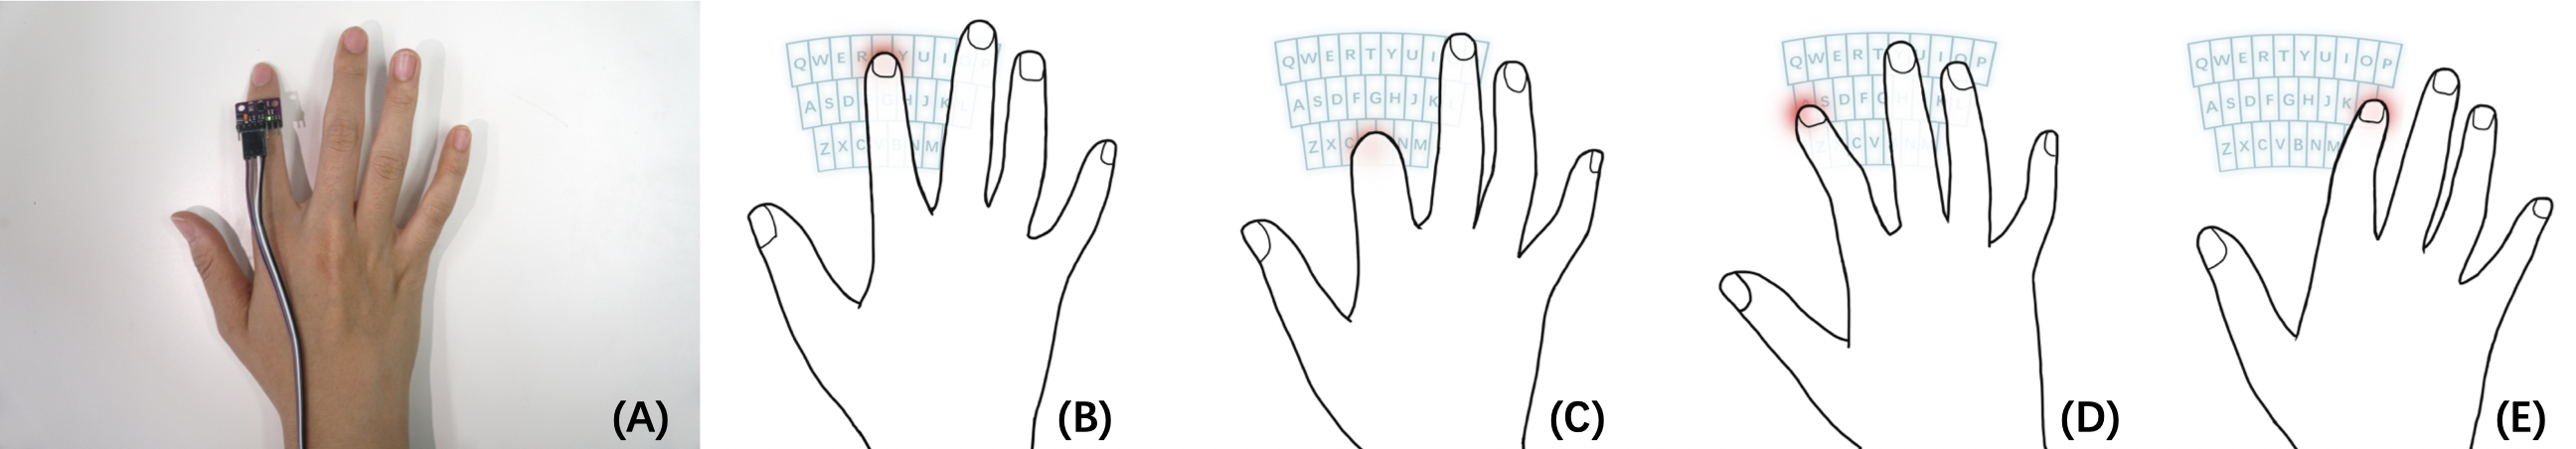
\includegraphics[width=1.0\linewidth]{QwertyRing_teaser.jpg}
	\caption*{用户将惯性传感指环佩戴在食指的第二指骨上,并将手腕放在无源交互表面上(图A),他想象在他的食指可触及的范围内有一个二十六键键盘(图B-E),然后打字。智能打字指环根据惯性传感数据识别触摸事件,并预测用户想要的单词。用户从任意显示设备(如显示器)接受视觉反馈。}
	\caption{智能打字指环的交互流程}
	\label{fig:QwertyRing_teaser}
\end{figure}

如图\ref{fig:QwertyRing_teaser}所示是智能打字指环的交互流程图,这是一种基于六轴惯性传感器指环的无源表面文本输入技术。智能打字指环适用于任意类似桌面的交互表面,交互表面要求是刚体的、平坦的、且足够宽敞,至少需要能够容纳一个手机的大小。用户通过触摸无源交互表面键入字符,并从单词推荐列表中选中所需的单词。在使用过程中,用户将惯性传感指环佩戴在食指的第二指骨上,并通过外部显示器(如混合现实头盔、增强现实头盔、智能电视)接受视觉反馈。用户将手腕轻放在交互表面上,想象其食指可触及区域内有一个二十六键键盘,然后打字。软件系统通过惯性传感指环的信号检测触摸事件,并根据指环在手指连续几次触摸中的方向预测用户所需的单词。

相比于头戴式显示设备上已有的文本输入方案,智能打字指环具有多重优势。首先,智能打字指环仅通过惯性传感指环采集用户打字信号,传感器的生产成本低、功耗低;其次,智能打字指环使用方便,该设备是可穿戴的,允许用户在任意类似桌面的无源表面上打字,具有很高的普适性;第三,用户在使用智能打字指环打字时不需要将注意力集中在手部,而可以专注在显示设备上,这一点对虚拟现实头盔和智能电视交互场景来说都是很重要的\cite{lu2017blindtype};最后,智能打字指环是易于学习的,由于它借鉴了手机软键盘的二十六键布局,保留了用户在日常打字过程中积累的关于打字的肌肉记忆。

现有文献尚未探索使用智能指环支持无源表面文本输入的可行性,这其中有一些挑战:首先,仅使用智能指环,而不辅以其它传感设备时,手指在交互表面上的2D位置估计往往是不准确的(误差大于1厘米)\cite{kienzle2014lightring};其次,虽然上一章提到,可以利用惯性传感指环识别无源表面上的触摸事件,但仍有许多触摸手势的识别未被支持,包括触摸表面的手指何时抬起、长按和滑动手势等等。为了解决上述问题并构建智能指环打字技术,我们进行了三项用户实验,用于回答以下三个研究问题:

\textbf{(1) RQ1):如何利用惯性传感指环识别多种触摸手势?}
实验一收集了被试的触摸交互数据,包括点击、长按和滑动等触摸手势。上一章所述的基于惯性传感指环的触摸识别技术已经支持了对点击触摸的支持,在此基础上,研究者根据触摸运动模型,支持对手指抬起事件的检测,准确率(F1综合评价指标)达到99.50\%。进一步地,基于对触摸事件和手指抬起事件的检测,系统可以通过简单的阈值方法识别其它触摸手势,包括长按、向左滑动和向右滑动。

\textbf{(2) RQ2):如何设计文本输入法的候选词解码器?}
实验二收集了被试使用智能打字指环在无源表面上打字的数据,基于数据,实验者分析了被试的打字行为,从而设计了智能打字指环的候选词解码器。候选词解码器是根据用户字符输入序列猜测用户所需单词的贝叶斯解码器。结合trigram[28]语言模型,解码器在模拟实验中有79..0\%的概率将用户所需单词预测为第一位候选词,有94.5\%概率将用户所需单词预测为前五位候选词。结果表明,该解码器有能力支持基于选词的文本输入方法。此外,实验者通过观察实验数据发现,被试们的打字行为之间存在较大差异,这启发实验者探索个性化文本输入模型。

\textbf{(3) RQ3):用户使用智能打字指环打字的速度有多快?}
实验三在使用通用候选词解码器和个性化解码器两种情况下,评测了被试使用智能打字指环进行文本输入的打字效率。实验三是为期五天的用户实验,评测了被试使用智能打字指环打字时的中短期学习效应。结果表明,无论是使用通用候选词解码器还是个性化解码器作为,智能打字指环的表现都是良好的。平均而言,被试在40分钟的练习之后就能达到每分钟输入13.74个英文单词的打字速度,在为期五天,每天打字40分钟的练习过后,其打字速度达到每分钟输入20.59个英文单词。从第三天开始,个性化候选词解码器呈现出由于通用候选词解码器的趋势(p=.09)。

本章工作的贡献有三个 方面:(1)首先,根据触摸运动模型,实现了在无源交互表面上的多手势触摸交互,包括对手指抬起事件、长按、左滑和右滑的识别,识别准确率超过99\%;(2)其次,本章介绍了仅使用单个惯性传感指环作为输入设备,支持无源表面上26键文本输入的方法;(3)本章通过实验证明,智能打字指环为混合显示头盔、智能电视等新型显示设备提供了实用、高效的文本输入方案。

\section{相关工作}

\subsection{可穿戴文本输入}

随着可穿戴设备与技术的发展,越来越多的研究者对可穿戴设备上的文本输入方法产生兴趣,利用可穿戴设备支持文本输入的用途很广泛,适用于多种新型显示设备,例如增强现实头盔和虚拟现实头盔\cite{yu2017tap, yu2016one}、大屏幕显示器\cite{markussen2013selection, schick2012vision}、智能手表\cite{oney2013zoomboard, yi2017compass},等等。

\subsubsection{智能手表文本输入}

利用可穿戴设备上的触摸屏是研发可穿戴文本输入的最直接方法,而智能手表是其代表性设备平台。“胖手指问题”是智能手表文本输入技术的主要挑战\cite{yi2017too}:由于智能手表触摸屏的空间有限,手表触摸屏中单个按键太小会导致用户无法准确点击的问题。对于字符级别的文本输入,一些技术采用多次点击确定单个字母\cite{chen2014swipeboard, hong2015splitboard, oney2013zoomboard}或区别对待不同手指点击\cite{gupta2016dualkey}的方法来克服“胖手指问题”,还有的技术则采取规避手指遮挡的策略\cite{leiva2015text, shibata2016driftboard}。尽管与上述工作类似的方法有很多,但是从信息论的角度来说,只要是小触摸屏上的文本输入方法,就会面临屏幕大小制约了文本输入速度上限的问题\cite{yi2017too}。此外,基于触摸屏的智能手表文本输入需要双手的参与,使其适用场景受限。

另有一部分智能手表上的文本输入技术不依赖触摸屏。COMPASS用户通过旋转智能手表的表圈进行文本输入\cite{yi2017compass},输入速度达到每分钟12.5个英文单词。WrisText用户通过手腕动作进行文本输入\cite{gong2018wristext},输入速度达到每分钟15.2个英文单词。以上技术不遵循广泛使用的文本输入交互规范(例如26键键盘和触摸交互),因此具有较高的学习门槛,不容易学习和走向实用。

\subsubsection{空中手势文本输入}

大部分基于空中手势的文本输入技术都依赖视觉方法追踪手部运动,它们适用于可穿戴场景,例如,混合现实头盔的前置摄像头可用于追踪手部运动。手部追踪技术支持了基于一笔画\cite{ni2011airstroke}、目标选择\cite{markussen2013selection}、滑动手势键盘\cite{kristensson2004shark2}和手写\cite{schick2012vision}的空中手势文本输入。对比上述工作发现,Qwerty二十六键键盘是基于目标选择的空中手势文本输入中最好的布局,可使文本输入速率达到每分钟18.9个英文单词\cite{markussen2013selection}。滑动手势键盘比基于目标选择的技术更适用于空中文本输入任务,输入速率达到每分钟28.1个英文单词\cite{markussen2014vulture}。然而,由于缺少物理支撑,基于空中手势的文本输入技术都会导致用户疲劳,影响长时间文本输入的体验。此外,文本输入需要高精度的输入信号,需要使用Optitrack\cite{point2011optitrack}等昂贵的摄像头设备进行准确的手部跟踪。因此,在目前的商用混合显示设备中采用空中手势文本输入方案是不切实际的。

\subsubsection{智能手套文本输入}

不少相关工作专门为文本输入设计了智能手套。基于智能手套的文本输入技术分为两种,分别是利用(1)空中手写,和(2)手指之间的敲击来输入文本。基于空中手写的技术是易于学习的\cite{amma2012airwriting, zhou2008hand},但是存在用户易疲劳的问题,而且,凡是基于手写的文本输入技术,都存在每分钟输入15个英文单词的打字速度上限\cite{devoe1967alternatives}。基于手指间敲击的文本输入法依赖特定的输入规则\cite{bajer2012huffman, goldstein1999finger, peshock2014argot, rosenberg1999chording, seibel1962performance, whitmire2017digitouch},因此学习门槛高是一个大问题。DigiTouch\cite{whitmire2017digitouch}是一个巧妙的设计,它将二十六键键盘的每个字母拆分映射到不同手指的各个指骨上,拇指点击相应指骨来输入文本。DigiTouch用户通过三个小时的练习,能够达到每分钟输入16.0个英文单词的输入速度,其结果是同类型工作中较为出色的。

\subsubsection{智能指环文本输入}

相关工作中基于智能指环的文本输入方法较少。一部分工作提出利用智能指环识别26个英文字母\cite{gummeson2014energy, zhang2017fingersound, zhang2018fingerping},然而,这些工作仍专注于提升将手势识别成英文字母的准确率上,准确率不超过93\%,这一准确率是无法支撑流畅的文本输入体验的。ThumbText是一款佩戴在食指上的小型触摸屏\cite{kim2018thumbtext},用户使用拇指分两步点击触摸屏来输入一个字母,专家用户的打字速度为每分钟输入11.4个英文单词。TipText是一个在食指第一指骨上的虚构软键盘\cite{xu2019tiptext},键盘布局是一个2乘3的网格,布局针对盲打进行过优化,专家用户的打字速度为每分钟13.3个英文单词。RotoSwype是一种基于惯性传感指环的指向的空中滑动输入键盘\cite{gupta2019rotoswype},经过五天的训练,用户的平均打字速度可以达到每分钟输入14.8个英文单词。

TypingRing\cite{nirjon2015MobiSys}与本章所介绍的技术最为相似,同为基于指环的无源表面文本输入技术,用户分两个步骤打字。TypingRing将二十六键键盘分为九个区域,每个区域包含三个按键。用户首先通过平移他们的手来选中一个区域,然后通过用食指、中指或者无名指触摸来三选一选出想要的字母。TypingRing存在一些不足:首先,分两个步骤进行的文本输入并不直观,打字效率也很低,该技术的专家用户打字速度为每分钟输入10.0个英文单词;其次,论文没有公布实验细节,无法判断实验是否规范;第三,该技术的触摸识别部分准确率仅为80\%,无法支持流程的文本输入体验。

\subsubsection{可穿戴文本输入小结}

除了以上研究工作以外,还有其它输入方式可用于支持可穿戴设备的文本输入。例如,头动\cite{yu2017tap}、倾斜设备\cite{partridge2002tilttype}、控制触摸压力\cite{zhong2018forceboard}、眼动\cite{kurauchi2016eyeswipe, majaranta2007text, sarcar2013eyek}和一维触摸屏\cite{yu2016one}都可用于打字。然而,基于触摸和二十六键布局的键盘仍然是当前智能设备上最常用的文本输入系统。因此,实用性研究应该尝试在触摸和Qwerty键盘布局的基础上研发文本输入技术,而本章所述的基于惯性传感指环的无源表面文本输入则是可行方法之一。

\subsection{智能指环交互}

智能指环是人机交互领域中一个快速发展的方向,2015年一份文献综述Digital Digits\cite{shilkrot2015digital}对智能指环相关工作做了全面分析,指出智能指环的三大功能。首先,智能指环的主要功能是传感超出人类手指感知范围的事物,例如手势识别\cite{gupta2018asterisk, ogata2012iring, tsukada2004ubi, van2011finders, zhang2017fingorbits, zhang2018fingerping}。第二,智能指环可向佩戴者提供信息,例如触觉反馈\cite{prattichizzo2010remotouch, solazzi2010design}。第三,人的手指可通过智能指环控制或发送信息到外部对象,例如智能指环控制系统\cite{ashbrook2011nenya, chan2013fingerpad, harrison2009abracadabra, nguyen20153dtouch}。大多数研究,包括本章所介绍内容,都是将指环作为传感设备。本节相关工作介绍将从手指跟踪和触摸检测两个方面讨论智能指环的识别能力。

\subsubsection{手型跟踪技术}

声学\cite{zhang2017soundtrak}和磁力学\cite{chan2013fingerpad, chen2013utrack, parizi2019auraring}都可以作为智能指环手型追踪技术的基本原理,但只能用于检测智能指环与其它手部穿戴设备之间的相对位置,其识别精度在4.4毫米到13毫米不等。AuraRing\cite{parizi2019auraring}是基于磁力学的智能指环手型跟踪技术中效果最好的,其识别精度为4.4毫米,然后,AuraRing的配置不仅包含一个指环,还包含一个带有多个传感线圈的腕带,这使得它在便携性上不如单指环系统一样出色。视觉方法同样可以支持智能指环手型追踪技术\cite{chan2015cyclopsring, stearns2018touchcam, yang2012magic},但他们存在遮挡、高功耗和高计算资源消耗等问题。惯性传感单元可以嵌入在智能指环中,用于跟踪手型,具有成本低、体积小、功耗低等优点。MIDS由智能手表外加两个带有惯性传感器的指环组成\cite{lam2002mids},LightRing由一个用于测量手指屈伸程度的红外接近光传感器和一个用于测量手指选择的陀螺仪组成\cite{kienzle2014lightring},它们都可以用户追踪手指在无源表面上的位置,但是精度降低且需要校准。
在我们的工作中,我们尝试使用单个 6 轴 IMU 来估计手指的弯曲和旋转。

\subsubsection{触摸识别技术}

智能指环可支持无源表面触摸识别技术,即识别手指触摸无源表面的交互事件。先前基于指环的工作仅利用阈值方法识别触摸事件\cite{lam2002mids, oh2017anywheretouch, masson2017whichfingers},准确率不超过89.8\%。直到如上一章所述,本文作者利于触摸运动模型改进指环触摸识别技术\cite{gu2019accurate},指环触摸识别的准确率才达到实用的级别(99.3\%)。然而,上一章内容仅支持了对手指接触无源表面瞬间的识别,不包括对手指触摸交互表面以后抬起事件的识别,也不包括对长按、滑动等多样化触摸手势的识别。与其它可穿戴文本输入技术\cite{xu2019tiptext, yi2017too, yu2017tap}一样,本章将要介绍的智能打字指环文本输入技术也需要包括长按和滑动在内的多种触摸手势来支持文本输入应用程序。因此,为了构建智能打字指环文本输入技术,本章还需先解决手指抬起事件的检测和其它触摸手势的识别问题。

\subsubsection{智能指环交互小结}

综合上述文献可以发现:(1)即使通过个性化的校准\cite{kienzle2014lightring},单个智能指环跟踪手指位置仍是不精确的,误差大于1厘米;(2)尽管本文第二章已经攻克了基于指环的低延迟触摸识别技术,但是对更多触摸手势的识别仍然需要进一步探索。鉴于现有工作存在以上不足,在构建智能打字指环之前本章必须先解决两个先决技术:(1)首先,使用贝叶斯解码器从不准确的输入信号中联想用户想要的单词。与许多其它依赖智能联想的文本输入技术一样\cite{gong2018wristext, gordon2016watchwriter, gupta2019rotoswype, markussen2014vulture},智能打字指环也无法支持词汇表外(OOV)的单词;(2)第二,研发可以检测无源表面上多样化触摸手势的技术,触摸手势包括手指抬起、长按、滑动,等等。

\subsection{贝叶斯解码器}

贝叶斯方法被广泛应用于文本输入解码器,用于通过输入信号联想用户所需单词\cite{goodman2002language},其基本思想是根据词语出现的概率(语言模型)和触摸点的分布(触点模型)来估计词库中每个单词作为用户想要单词的概率,从而将概率最大的单词上屏,或者将概率最大的若干候选词展示出来供用户选择。对于语言模型,本章将评估一元、二元和三元模型\cite{ide2008american}对单词联想准确率的影响。对于触点模型,大多数文本输入研究假设每个按键上的触摸点云服从二维高斯分布,这是绝对触点模型\cite{azenkot2012touch, goodman2002language}。然而,BlindType这篇论文\cite{lu2017blindtype}指出,当用户在文本输入中手眼分离时,连续触点之间的向量也服从二维高斯分布,这是相对触点模型。

\section{智能打字指环的交互设计}

本节首先介绍无源表面指环文本输入技术(智能打字指环)的交互设计,包括硬件配置、键盘布局和交互流程;然后,本节再介绍设计准则,即为什么要采取所述交互设计。在硬件上,智能打字指环是嵌入了六轴惯性传感的智能指环,交互时用户将指环佩戴在食指第二指骨上。如图\ref{fig:QwertyRing_teaser}A所示是智能打字指环的交互流程:用户将手腕放在桌子上,想象在其食指可触及区域内有一个Qwerty二十六键键盘。用户不能真的在桌面上看到一个二十六键的键盘布局,而是仅凭想象判断二十六个英文字母按键的位置,因此本节将此键盘成为想象的二十六键键盘。用户通过额外的显示设备来查看键盘布局。为了减少用户定位想象键盘上每个字母位置的认知负担,键盘的26个按键被设计成占满了食指的整个可触及区域,图\ref{fig:QwertyRing_teaser}B-E展示了想象键盘的边界:第一排键位位于食指指腹的最远触摸范围上;第三排键位位于食指指尖轻敲的位置上;键盘的左右边界刚好在用户转动手腕时食指能够轻松够到的范围内。

\subsection{键盘布局}

\begin{figure}
	\centering
	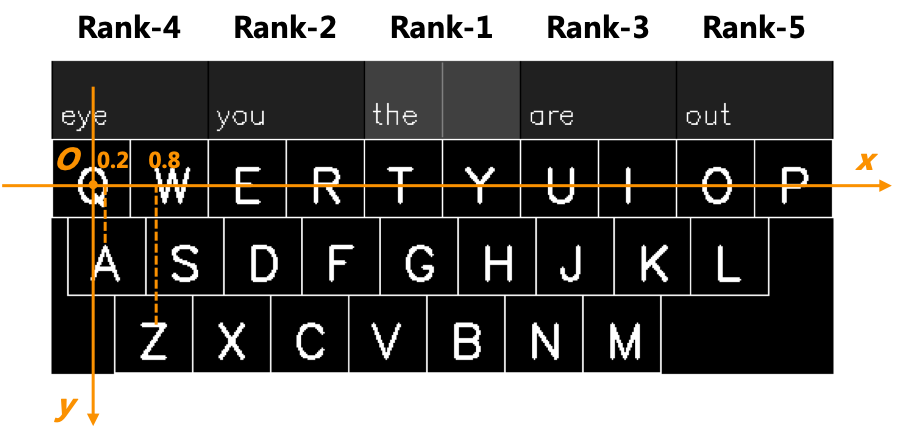
\includegraphics[width=1.0\linewidth]{QwertyRing_layout.png}
	\caption*{图中展示了智能打字指环的键盘布局,Rank-1表示最有可能的候选词。字母Q、A、Z
		、P、M的中心坐标位置是(0,0)、(0.2,1)、(0.8,2)、(9,0)和(6.8)。}
	\caption{智能打字指环的键盘布局}
	\label{fig:QwertyRing_layout}
\end{figure}

用户从外部显示器(例如增强现实头盔、显示器或智能电视)观看如图\ref{fig:QwertyRing_layout}所示的键盘布局作为视觉反馈。键盘由二十六键布局图和候选词选择区域组成。二十六键布局图的作用是提醒不会盲打的用户26个字母按键所在的位置。在文本输入的过程中,系统将始终预测当前输入序列对应的前五名候选词,显示在候选词选择区域上,从左到右的候选词排序是第四名、第二名、第一名、第三名、第五名候选词。也就是说,最有可能的候选词是放在中间的,次有可能的候选词放在两边,这一设置旨在节省选择单词所需的时间。在文本输入的过程中,用户可以将注意力集中在显示器上,而不需要将注意力放在自己的手上。

\subsection{交互流程}

用户按以下步骤输入单词:

\begin{enumerate}
\item 在想象的二十六键键盘上按顺序点击所想单词的每个字母。
\item 长按200毫秒触发候选词选择功能,先不抬起手指,这时在Rank-1候选词上会出现一个光标。
\item (可选)若Rank-1候选词不是想要的单词,通过左右滑动控制光标选择其它单词。当指环沿着竖直轴旋转7.5° 时,光标移动一格。
\item 抬起手指选中光标所在的候选词上屏。
\end{enumerate}

用户通过左滑手势删除单词。与许多其它依赖智能联系的文本输入技术一样\cite{markussen2014vulture, yi2017compass, yu2017tap},如果用户所需单词不在候选词列表中,用户需要删除错误的单词,重新输入。在使用智能打字指环输入文本时有一个限制,由于指环上的惯性传感器只能传感食指的指向,但不能传感手指的平移,因此用户需要将手腕放在交互表面上不要平移,只通过转动手腕来触及不同的按键。只有有了这个约束,惯性传感指环才可能区分同一行的不同键位。用户需要一些时间的熟悉来适应这一要求,本章将在后面讨论熟悉阶段的学习效应。

\subsection{设计准则}

本小节将讨论智能打字指环的设计准则,即对本技术的交互设计细节做出解释。以下讨论可能会涉及到实验二的结论,该实验收集并分析了用户的打字数据,读者可以在后面的第4.5节找到有关实验二的详细信息。

{(1)为什么使用长按、滑动等触摸手势选词和删除单词,而不使用按钮?}:在智能打字指环的键盘布局中,26个键已经占满了整个食指的可触及区域,因此,没有额外的空间来安放进入用于选词的数字按钮和删除单词按钮。首先,这一设计降低了用户在定位所想字母时所需要的认知负担,例如,因为在26键的上方没有数字按钮,所以用户在输入键盘中第一行的字母时,只需将手指尽可能伸直,而无需担心手指点中了数字按钮;其次,这一设计提高了单词联想的准确率,因为先前工作已经证明,小屏幕文本输入中键盘布局越大,单词联系的准确率也越大\cite{yi2017too}。

{(2)为什么可选的候选词是五个?}:一方面,如果候选词较少,则用户想要的词很有可能未出现在候选词列表中。根据实验二的模拟实验结果,单词解码器将用户所需单词排在候选词前五名的概率为97.5\%,而排在前三名的概率仅为93\%。如果用户所需单词不在候选词列表中,用户只能重新输入,影响打字效率。另一方面,如果候选词较多,用户在选词过程中,可能会因为对手指指向控制不够准确而选错单词。综合上述原因,五个候选词是交互效率最高的选择。

{(3)为什么选词过程中,手指旋转7.5°对应光标移动一格候选词?}:实验二收集了用户使用智能打字指环打字时的数据。数据分析显示,被试手腕舒适的左右旋转角度在30° 左右,因此,智能打字指环将候选词区域中的五个格子映射到-15°、-7.5°、0°、7.5°和15°的手指左右选择角度上。

{(4)为什么将智能指环佩戴在食指第二指骨上?为什么要求用户在打字的时候手腕不能平移?}:首先,这两条约束性的交互设计对于智能打字指环的单词联想来说是必须的,智能打字指环的工作原理是将惯性传感指环的方位角(偏航角和俯仰角)映射到键盘布局的X轴和Y轴上的。如果将智能指环佩戴在食指第一指骨上,用户打字过程中无论手指点击哪一行,智能打字指环的俯仰角都不会发生很大的变化,因此指环信号不能提供用户点击了哪一行字母的有效信息;如果用户在打字过程中通过手腕左右平移来点击不同列上的字母,则智能打字指环的偏航角不会发生很大变化,无法提供用户点击了哪一列字母的有效信息。其次,这两条约束性的交互设计对用户的主观体验而言尚可接受。上一章的指环佩戴位置主观喜好程度调研发现,智能指环最被用户接受的佩戴位置是手指的第一指骨,其次第二好的就是第二指骨了。手腕不允许平移的设计也是可以接受的,本章的实验二发现,手腕左右旋转在30°的范围内是舒适的。

\section{指环上的触摸手势识别}

\subsection{实验一:收集触摸手势数据}

实验一收集被试佩戴惯性传感指环在桌面上触摸交互的数据,包括点击、长按、滑动等交互任务。实验的动机是为触摸手势识别技术的研发提供数据支持。在此,本节先对手指的触摸事件和抬起事件给出明确的定义:\textbf{触摸事件}指的是触摸交互中,手指接触到交互表面的一瞬间。在手指接触到交互表面以后,手指可能立即抬起,也可能在停留等待或在平面上移动过后再抬起。\textbf{抬起事件}指的是手指触摸交互表面后,离开交互表面的瞬间。本节将分三个步骤探索触摸手势的识别问题:

(1)对于\textbf{触摸事件},其识别方法已经在上一章详细介绍了,本节将简要回顾。

(2)对于\textbf{抬起事件},本节将结合触摸运动模型,设计抬起事件的识别算法。

(3)基于对触摸事件和手起事件的识别,本节采用机器学习支持了对\textbf{长按、左滑、右滑}等触摸手势的识别。

\subsubsection{实验设计和过程}

实验者从大学校园中招募了12名被试参与实验,被试的年龄从19岁到25岁不等,平均年龄为21.59岁,标准差为2.02岁,其中4名被试为女性。所有被试都是右撇子。如图\ref{fig:QwertyRing_config}所示实验一的实验设置,在木质的桌子上固定着一块薄而坚硬的触摸板。被试将惯性传感指环佩戴在食指的第二指骨上,并在触摸板上执行实验要求的各种触摸手势。实验任务是实验者口头传达的,共包含四组数据集的收集:点击、长按、滑动和空中手势。其中,点击、长按和滑动用于采样各种触摸手势下的触摸事件和抬起事件的信号样本,而空中手势则作为触摸事件的负样本。

\begin{figure}
	\centering
	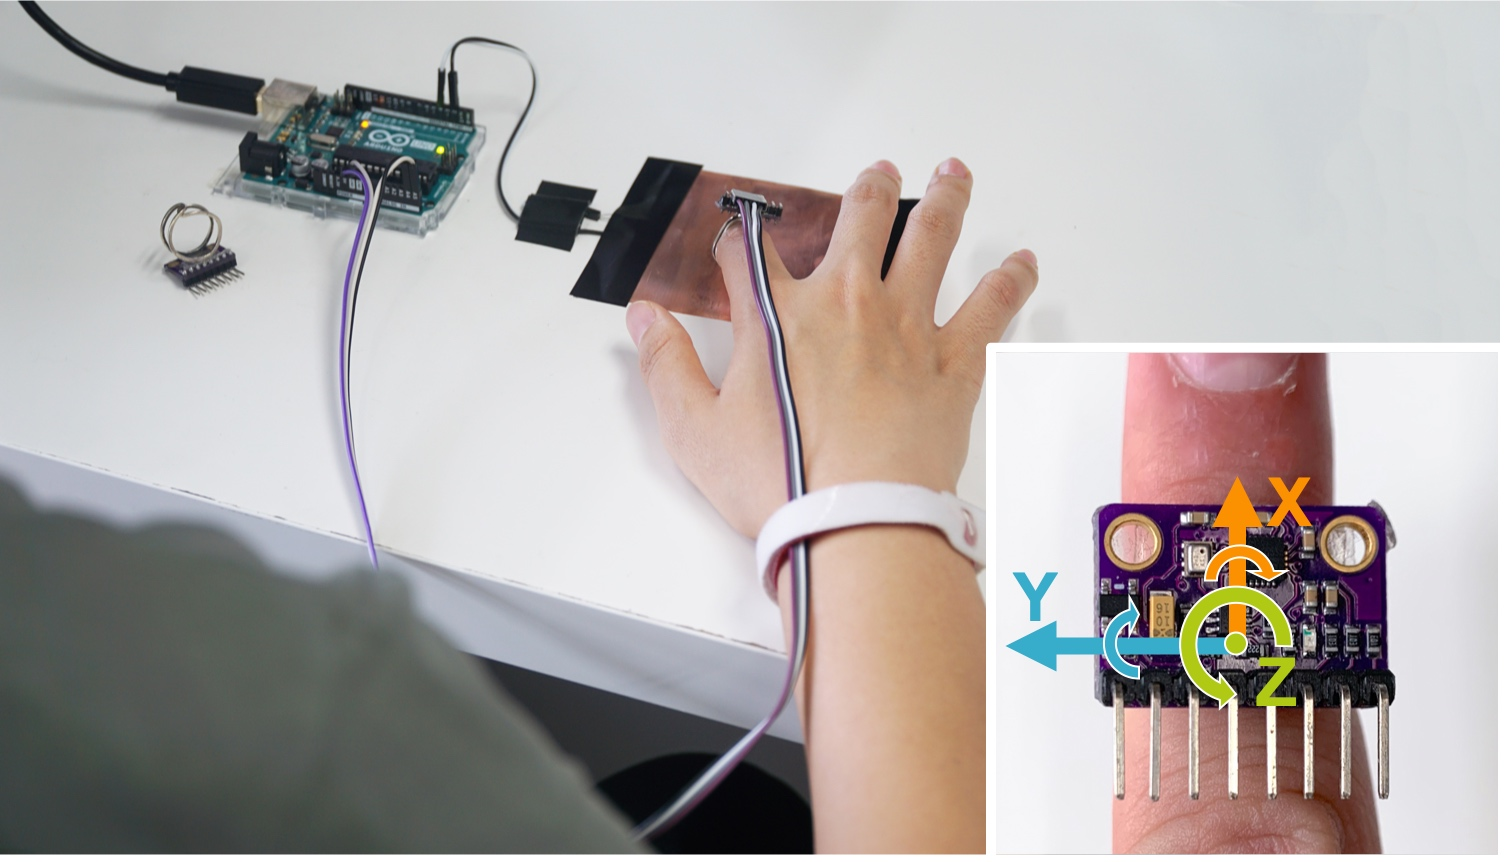
\includegraphics[width=0.8\linewidth]{QwertyRing_config.jpg}
	\caption*{图中展示了实验一的实验设置,小图展示了惯性传感指环的佩戴位置和指环的坐标轴。}
	\caption{实验一的实验设置}
	\label{fig:QwertyRing_config}
\end{figure}

\textbf{(1)点击数据集}:被试在触摸板上点击5组$\times$100次=500次。被试以自己喜欢的方式以任意的触点位置、触摸力度和角度进行点击,实验共收集了来自12名用户的6000次点击样本。

\textbf{(2)长按数据集}:被试在触摸板上长按5组$\times$100次=500次。在长按过程中,被试可以自行选择将手指保持不动,或者在交互表面上移动手指。

\textbf{(3)滑动数据集}:被试共执行了10组$\times$100次=1000次滑动手势,包括5组左滑和5组右滑。实验者要求被试想象自己像在智能手机上切换屏幕一样去执行滑动手势。在收集点击数据集、长按数据集和滑动数据集的过程中,被试需要将手腕休息在桌子上,不能平移手腕,这一要求与智能打字指环的交互流程保持一致。

\textbf{(4)空中手势数据集}:被试在一分钟的时间内,根据实验者的口头指令,在空中做出五种空中手势。手势分别是在空中保持不动、在空中左右滑动手指、画圆、画正方形和手指剧烈颤抖。这些空中手势是触摸事件的负样本,特别是手指剧烈颤抖的信号,是波形最接近触摸事件的空中手势信号,这说明本数据集是非常严格的。

在每两组实验之间,被试被要求休息一分钟,以避免疲劳。本实验的总时长大约为一小时。

\subsubsection{实验设备}

本实验的实验设备如图\ref{fig:QwertyRing_config}所示。其中,惯性传感指环由GY-91惯性传感器和普通的装饰性指环粘合而成。为了让智能指环适合不同手指粗细的用户,实验者共制作了四枚大小不一的惯性传感指环,供用户选择。惯性传感单元通过杜邦线连接到Arduino(Uno R3)开发板上。实验者用魔术贴将杜邦线固定在被试的手腕上。该指环收集六轴的运动信号,包括原始加速度和角速度。其中,原始的加速度信号是线性加速度和重力混杂的结果,系统通过Madgwick滤波器\cite{madgwick2010efficient}将原始加速度分解为线性加速度和重力。实验中并未收集惯性传感指环的磁力计数据,这是因为磁力计的采样频率太低,而且容易受到周围设备的影响。图\ref{fig:QwertyRing_config}中的触摸板是一块连接到Arduino开发板上的导电铜片。当被试的手指接触到导电铜片的时候,手指与铜片形成耦合电容,电容增大,该实验系统利用这一现象来判断手指是否接触到交互表面\cite{badger2018capacitive},作为实验的真值。以上实验设置与上一章中的数据收集实验的设置很类似,但数据收集的性能得到了很大的改进,惯性传感指环和触摸板的传感频率都达到了1000赫兹,触摸板的识别延迟低于1毫秒。这些数据采集性能的提升来自采样代码的优化、实验主机性能的提高和交互表面的小型化。最终,实验共收集了11个维度上的运动数据,包括时间戳、三轴线性加速度、三轴角速度、三轴重力(方向)和触摸事件的真值。

\subsection{触摸手势识别技术}\label{section:model_QwertyRing}

\subsubsection{触摸检测}

触摸事件指的是触摸交互中,手指接触到交互表面的一瞬间。虽然上一章已经详细介绍了基于惯性传感指环的触摸事件识别技术,但是本章仍然回顾并在新的数据集上重新评测该技术。这是因为本章所采集的数据与上一章有所不同,更具有多样性(包含各种触摸手势)、采样频率更高、无位移信号、惯性传感指环佩戴在食指的第二指骨上,这些都是上一章没有评测过的情况。

实验者沿用第\ref{section:TappingRing}中章低延迟触摸识别技术的代码,修改程序使之适应于1000赫兹的惯性传感信号,然后用实验一收集的数据对该技术进行评测。结果表明,触摸识别技术在本数据集下的召回率为99.37\%(SD=0.94\%),精准率为99.24\%(SD=1.03\%),平均延迟为14.04毫秒(SD=7.40)。该结果在准确率上与上一章结果(表\ref{tab:tapping_ring_study3})相比差异不大,这是因为本实验所采集的数据采样频率更高,但没有基于视觉的手指位移数据,这两点因素一正一反地影响了触摸事件识别的准确率。该结果与上一章结果相比延迟多了5毫秒,这一差异不是技术实现造成的,而是因为本实验的实验数据包含了左滑和右滑的数据。在这两种触摸手势下,由于用户在组织手指运动时,有部分的力量花在了手指运动的水平分量上,使得在手指运动在垂直方向上不如直接的点击运动快速,根据触摸运动模型对触摸识别技术的指导意义(第3.8.1小节),这种情况下的识别延迟的确会增大。在误触率方面,该技术在12名被试共60分钟的空中手势数据集中仅触发了14次误触事件,这说明,即使用户在空中做出诸如剧烈抖动手指等接近触摸碰撞的空中手势,该触摸识别技术依然不会轻易引发误触。

\subsubsection{触摸与抬起的相关性}

\textbf{(1)大多数情况下,触摸发生在触摸运动中点$\frac{t_1}{2}$之前,抬起发生在中点之后}。

%识别触摸事件和抬起事件,其中,\textbf{触摸事件}是手指接触交互表面的瞬间,第\ref{section:TappingRing}章已经详细介绍了触摸事件的识别技术;\textbf{抬起事件}是手指触摸交互表面后,离开交互表面的瞬间,本章将详细介绍抬起事件的识别技术。在准确识别触摸事件和抬起事件以后,其它触摸手势的识别能通过简单的阈值方法解决,例如,长按手势等价于触摸和抬起之间的时间间隔超过一定阈值;左滑手势等价于从触摸到抬起手指向左移动超过一定阈值。

%基于最优控制理论的触摸运动模型只包含手指的向下运动过程,不包含对手指抬起的描述。尽管如此,触摸运动模型仍能为抬起事件的识别提供优化思路:对于点击和滑动等短时触摸交互而言,触摸交互中手指的向下运动过程和抬起过程有很强的相关性,主要体现在时间节点和运动速度这两方面。

如图\ref{fig:touch_up_model}所示,触摸运动模型蕴含了触摸时间$t_c$、触摸运动中点$\frac{t_1}{2}$和抬起时间$t_{up}$的关系:

\begin{equation}
	t_c<\frac{t_1}{2}<t_{up}
\end{equation}

其中,触摸运动中点$\frac{t_1}{2}$是触摸运动方程总时长的一半,也是人对手指的控制从向下加速到向上减速变化的瞬间:

\begin{equation}
	\begin{cases}
		a(t) < 0 & t < \frac{t_1}{2} \\
		a(t) \geq 0 & t \geq \frac{t_1}{2} \\
	\end{cases}
\end{equation}

根据第\ref{section:model}章的实验数据,在点击和滑动等短时触摸交互中,$t_c<\frac{t_1}{2}$成立的比例为92.86\%。也就是说,大多数触摸运动都是一个手指向下加速过程,在手指还未开始减速时,手指已经因为接触交互表面而瞬停。

根据第\ref{section:model}章的实验数据,在点击和滑动等短时触摸交互中,$\frac{t_1}{2}<t_{up}$成立的比例为96.45\%。这一现象可由触摸运动模型解释:当$t<\frac{t_1}{2}$时,人仍然对手指施加着一个向下的力,此时即使手指已经因为交互表面的阻挡而急剧减速,但尚不会反向运动离开交互表面;而当$t>\frac{t_1}{2}$时,人对手指施加的力转向向上,随后手指的运动才可能转向向上。这一规律对触摸抬起事件的识别有很大帮助,本章中后续介绍的实验证明,该判据有效降低了抬起事件识别的误报率。

\textbf{(2)触摸速度与$v(t_c)$与抬起速度$v(t_{up})$之间存在正相关性}。

\subsubsection{触摸与抬起的运动速度}

\begin{figure}
	\centering
	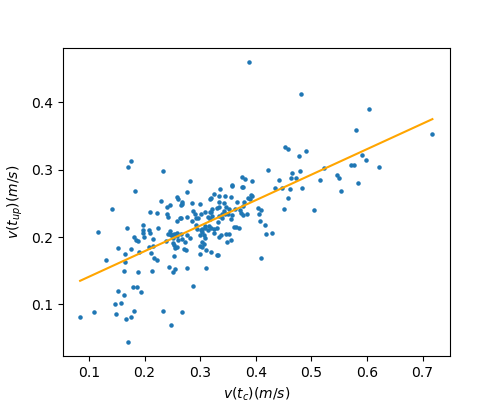
\includegraphics[width=0.6\linewidth]{vdown_vs_vup.png}
	\caption*{触摸与抬起的运动速度之间存在着正相关关系,因此触摸速度可以作为抬起事件识别的辅助判据。}
	\caption{触摸与抬起速度之间的关系}
	\label{fig:vdown_vs_vup}
\end{figure}

对于点击和滑动等短时触摸交互而言,手指向下点击的速度与抬起速度之间存在正相关的关系。如图\ref{fig:vdown_vs_vup}所示,根据第\ref{section:model}章收集的实验数据,触摸瞬间手指的速度$v(t_c)$与抬起瞬间手指的速度$v(t_{up})$之间存在关系:

\begin{equation}
	v(t_{up})=0.38\times v(t_c)+0.10
\end{equation}

其中,线性拟合的决定系数(R2)为0.48,说明$v(t_c)$与$v(t_{up})$之间存在弱相关性。因此,触摸速度这一信息可以作为抬起事件识别的一个辅助判据。

为了验证本文模型对触摸手势识别的优化是否实际有效,本章将基于上述优化思路,实现一种指环上的高效打字技术,该技术涉及到点击、长按、左滑和右滑等多种触摸手势。文本输入作为最快速、最复杂的触摸交互任务之一,可以严格地验证本章触摸识别技术的可用性。

\subsubsection{抬起事件识别}

抬起事件指的是手指触摸交互表面之后,离开交互表面的瞬间。抬起事件识别技术不仅要准确的、高响应地识别手指离开交互表面的瞬间,还要防止在手指接触着交互表面时,将手指在表面上的移动误识别成抬起事件。虽然触摸识别模型不包含对手指抬起过程的描述,但是该模型仍然对抬起事件的识别具有指导意义。

\begin{figure}
	\centering
	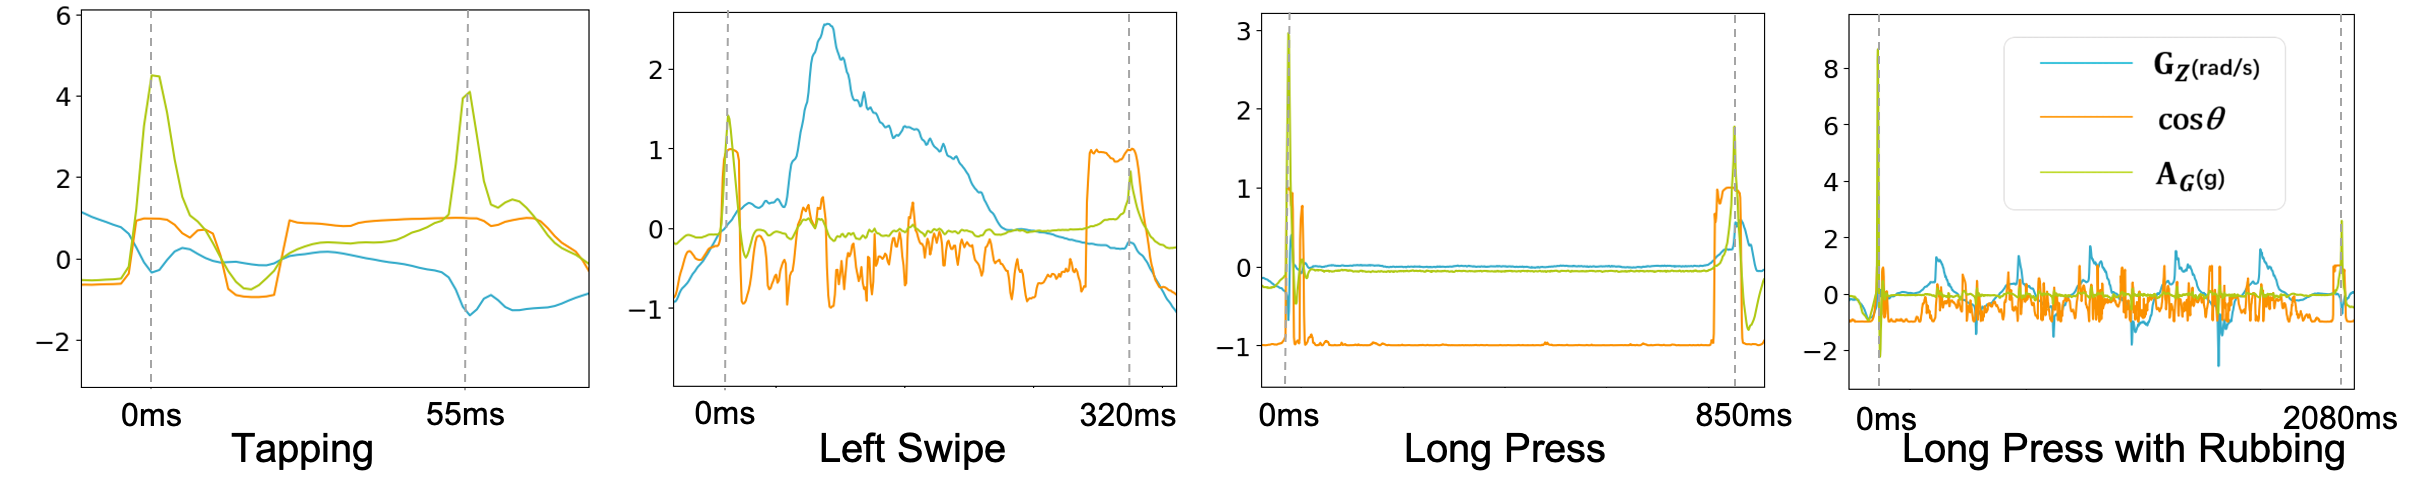
\includegraphics[width=1.0\linewidth]{touch_up.png}
	\caption*{图中展示了四种触摸手势下,从手指开始下落到最终离开交互表面的时间内,惯性传感器的相关信号。四种触摸手势分别是点击、左滑、长按和长按并晃动。}
	\caption{触摸交互信号图示}
	\label{fig:touch_up}
\end{figure}

如图\ref{fig:touch_up}所示是一次完整的触摸交互的相关信号,从左到右四幅子图分别是点击、左滑、长按和长按并晃动手指这四种情况下的惯性传感器相关信号,每幅子图中有两条竖虚线,表示触摸事件和抬起事件的发生时间。图中的三条曲线并不是指环上惯性传感器的原始信号波形,而是经过了提炼的,能够较好地检测抬起事件的特征值的曲线。绿线$A_G$是线性加速度在重力方向上的投影,相当于触摸运动模型中,手指与交互表面距离$x$对时间的二阶导。$A_G$在触摸事件和抬起事件发生的两个时间点上的振幅很大,波峰也十分尖锐。橙线$cos_\theta$是加速度方向和重力方向的夹角的余弦值,蓝线$G_z$是手指方位角上的角速度。从图中的波形可以看出,上述三个值都在手机抬起时具有明显的特征,可用于识别抬起事件。

然而,仅根据惯性传感器信号和上述指标识别抬起事件,准确率仍然较低。为了提高抬起事件的识别准确率,此处引入本章引言中提到的基于触摸运动模型的两条优化思路:

\textbf{(1)大多数情况下,抬起事件出现在触摸运动中点之后,即$t_{up}>\frac{t_1}{2}$。}这一规律可以有效处理指环上的抬起事件识别所面临的一个现实工程问题,即惯性传感器在遭到强烈震动(如手指接触交互表面)后,其信号会有10到30毫秒的时间处于紊乱状态。实验者推测,该紊乱状态是由惯性传感器自身原理和Madgwick滤波器共同造成的,难以避免。在这短暂的紊乱时间内,其信号很容易被误识别为抬起事件。根据公式$t_{up}>\frac{t_1}{2}$,实验者将当前时间$t$和触摸运动中点$\frac{t_1}{2}$这两个值也加入到识别抬起事件的特征组之中,如此一来,只要触摸运动的进度未过半,惯性传感器的紊乱就不太可能导致抬起事件的误报。

\textbf{(2)触摸速度$v(t_c)$与抬起速度$v(t_{up})$之间存在正相关的关系。}根据这一规律,实验者将手指触摸瞬间的运动速度$v(t_c)$也加入到识别抬起事件的特征组之中,如此一来,重触带来的大幅度信号紊乱更不可能引发抬起事件的误报,而轻触之后的抬起事件识别也能更为敏锐。

%。如图\ref{fig:touch_up_model_bk}所示,从触摸运动模型可以推断,手指抬起的时间$t_{up}$必然大于触摸运动主观时长$t_1$的一半,即$t_{up}>\frac{t_1}{2}$。这是因为,触摸运动方程揭示:当$t<\frac{t_1}{2}$时,人仍然对手指施加着一个向下的力,此时即使手指已经因为交互表面的阻挡而急剧减速,但不可能反向运动离开交互表面;而当$t>\frac{t_1}{2}$时,人对手指施加的力转向向上,随后手指的运动才可能转向向上。根据这一规律,实验者将$t$和$\frac{t_1}{2}$这两个量也加入到识别抬起事件的特征组之中,如此一来,只要触摸运动的进度未过半,惯性传感器的紊乱就不会导致抬起事件的误报。
%为了解决这一问题,实验者将$T_{escape}$也添加为判断手指抬起事件的指标,该值的含义是从手指触摸算起到当前时刻的时长。如图\ref{fig:touch_up_model}所示,根据触摸运动模型,在时间点$t=0$用户产生触摸意图,在时间点$t=t_c$手指接触到交互表面,而直到$t=t_1(t_1>t_c)$用户才从主观上认为向下触摸过程已结束,因此,在时间点$t=t_1$之前,手指是不会抬起的;只有当$T_{escape}>t_1-t_c$时抬起事件才有可能发生。加上这一限制能够有效缓解信号紊乱时期容易出现误识别的问题。

综上所述,本章采用触摸运动模型与机器学习相结合的方式来识别抬起事件:对50毫秒内的信号时间序列,提取21维特征向量,包含$A_G$、$cos_\theta$、$G_z$的最小值、最大值、均值、偏度和峰度,外加$t$、$\frac{t_1}{2}$和$v(t_c)$这三个值。其中,$t$、$\frac{t_1}{2}$和$v(t_c)$可以通过第二章所述的触摸运动模型的计算方法获取。实验者从点击、长按和滑动数据集中采样训练数据,正样本来至触摸手指抬起时刻周围的时间窗口[-25ms, 25ms],共24000份正样本。由于抬起事件识别的误触发指的是错把手指接触着交互表面时的动作误识别为抬起事件,因此负样本从手指接触着交互表面时的数据中随机截取。实验者从每一次的触摸数据中随机切取三段50毫秒的信号作为负样本,总共收集到54000个负样本。最后,基于上述正负样本数据,实验者采用简单的机器学习方法支持向量机(SVM)训练了一个二分类模型,模型的输入时任意50毫秒的21维特征向量,输出是这50毫秒的结束时刻是否发生了抬起事件。

留一(被试)交叉验证显示,模型在点击、长按和滑动数据集上预测抬起事件,召回率分别为98.61\%(SD=1.87\%)、99.68\%(SD=1.02\%)和99.53\%(SD=1.39\%),精准率分别为99.82\%(SD=0.24\%)、99.78\%(SD=0.31\%)和99.65\%(SD=0.42\%),识别延迟分别为8.55 毫秒(SD=4.97)、7.83毫秒(SD=3.47))和 7.97毫秒(SD=3.77)。结果表明,上述结合了机器学习和触摸运动模型的抬起事件识别模型,在预测准确率和延迟上都达到了较高的水平。

\subsubsection{长按}

基于触摸事件和抬起事件的识别,实验者采用阈值方法识别长按手势:当用户的手指接触交互表面并停留超过200毫秒时,系统报告长按事件。其中,停留值得是没有发生手指抬起事件,且手指上惯性传感指环的角速度始终小于0.1 rad/s。角速度的阈值是一个经验值,它确保大多数滑动手势不会被误识别成长按。为了评测上述长按识别方法的性能,实验者从长按数据集中采样正样本,从点击和滑动数据集中采样负样本。最终,留一(被试)验证法显示,该识别方法的召回率为98.8\%,精准率为99.2\%。后续的文本输入实验也进一步说明,本长按识别方法在实用中不存在任何问题。

\subsubsection{左滑和右滑}

由于长按事件已经被准确识别,所以接下来只需要区分点击、左滑和右滑三种触摸手势即可。实验者设计了两个特征来对上述三种触摸手势进行分类:触摸持续时长和旋转角度。图\ref{fig:swipe_feature}对比了点击、左滑和右滑三种触摸手势下,触摸持续时长和旋转角度的差别。从图中可以看出,三种触摸手势在上述两个特征的笛卡尔积平面上的点云是相互远离的,因此,一个简单的KNN(K=10)模型就可以准确区分这三种触摸手势。留一(被试)交叉验证法显示,该模型的三分类准确率为99.38\%(SD=0.43\%)。在实际使用中,系统将在检测到抬起事件时调用此三分类模型,判断用户是否执行了左滑或右滑触摸手势。

\begin{figure}
	\centering
	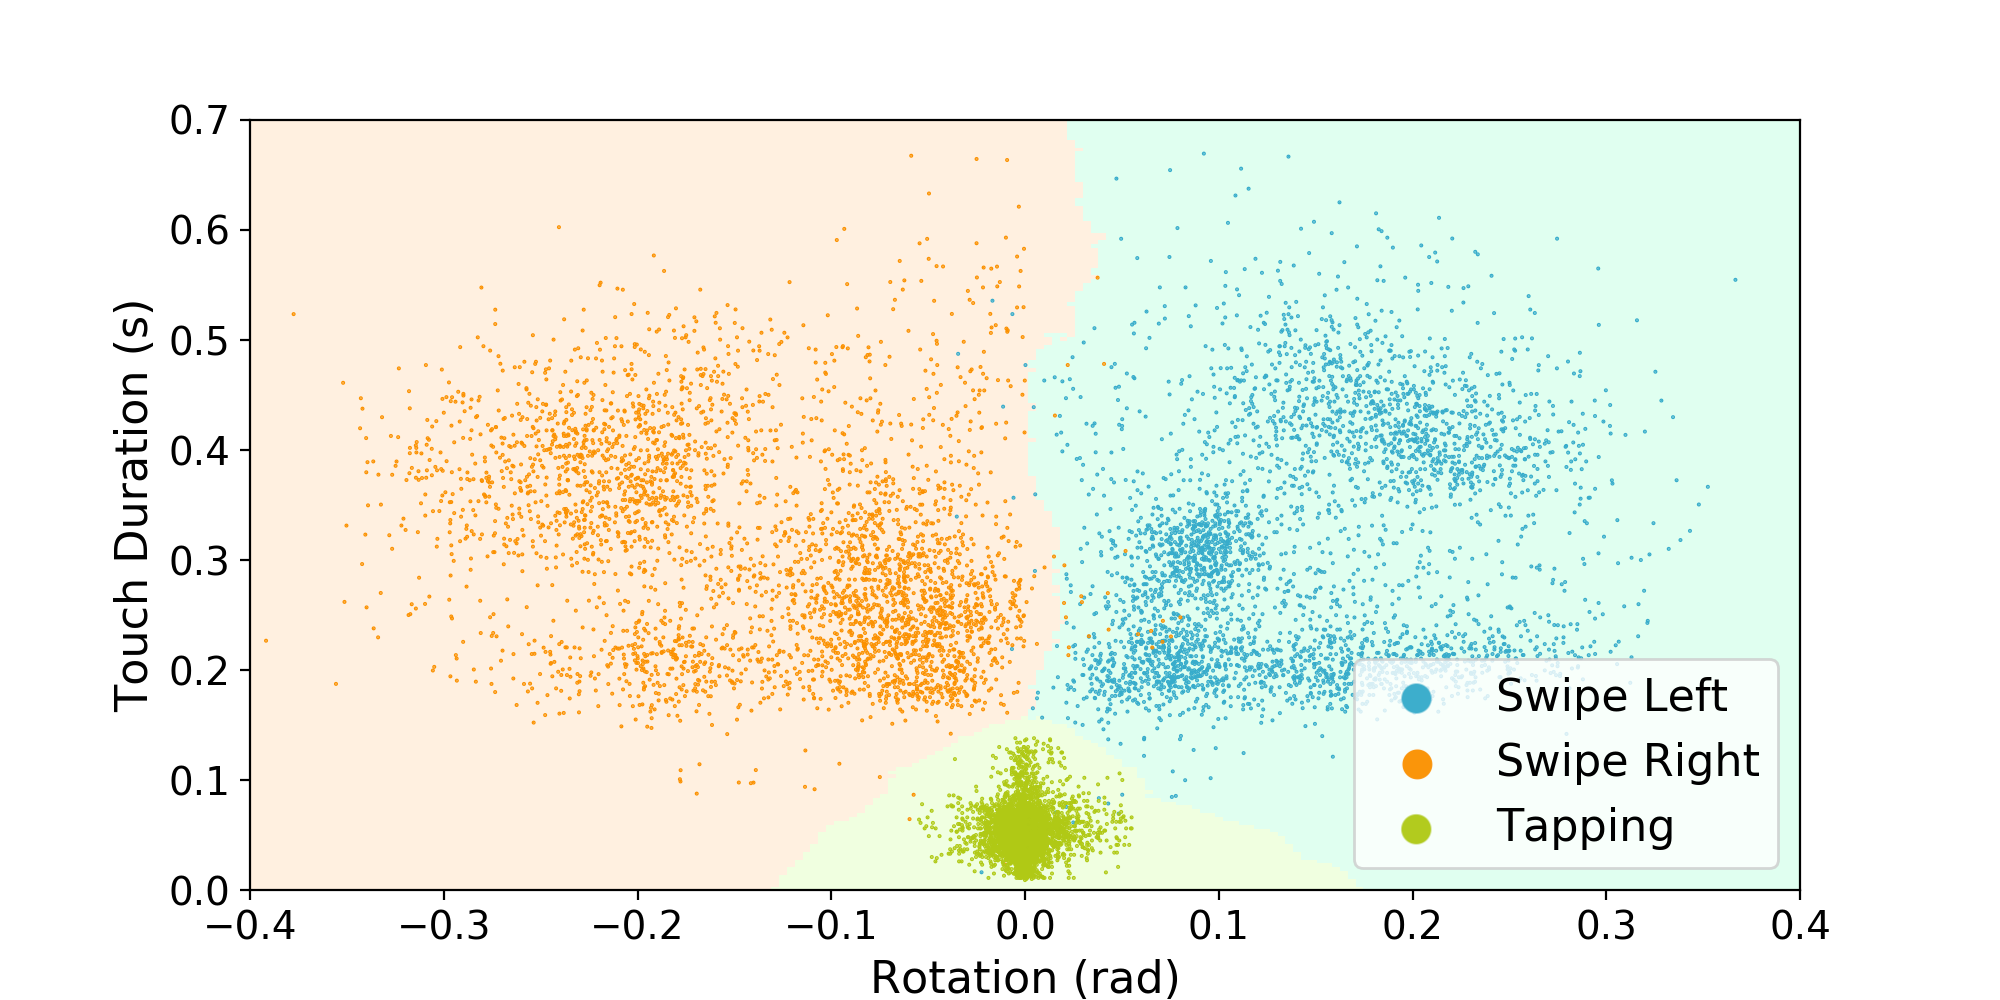
\includegraphics[width=0.8\linewidth]{swipe_feature.png}
	\caption*{如图所示是点击、左滑、右滑三种触摸手势在触摸持续时长和旋转角度这两个特征的笛卡尔积表面上的点云分布图,从图中不难发现,基于触摸持续时长和旋转角度这两个特征的KNN模型将能准确分类点击、左滑和右滑。}
	\caption{点击、左滑、右滑三分类模型}
	\label{fig:swipe_feature}
\end{figure}

\subsubsection{不同表面的触摸手势识别}

上述研究评测了触摸手势识别技术在木质桌面上的表现。在之前的数据采集实验中,实验者收集了被试佩戴运动传感指环在木质桌子上的触摸交互数据,桌子上还附有一块薄铜片,作为收集触摸与否的真值的触摸板。然而,之前的实验方法无法完美还原用户在无源表面上触摸交互的情形,因此,实验者进行了一项额外的实验,以在不同的无源表面上评测触摸手势识别算法,无源表面包括木质桌面(无薄铜片)、塑料桌面和人的大腿上侧(如图\ref{fig:study_over_surface}所示)。

\begin{figure}
	\centering
	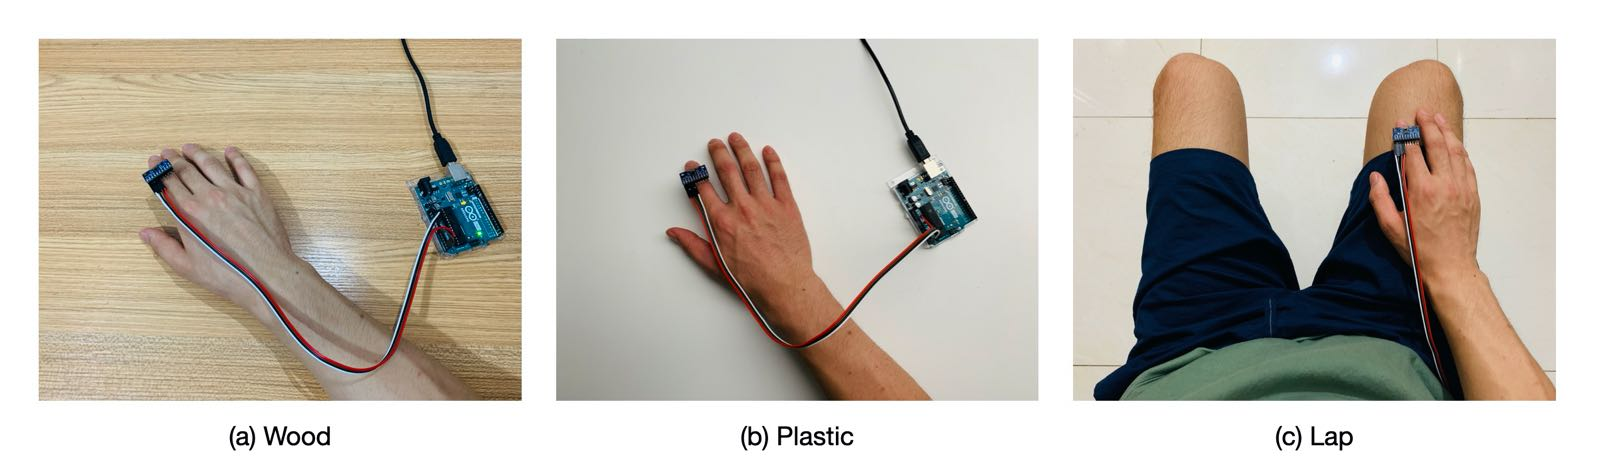
\includegraphics[width=1.0\linewidth]{study_over_surface.jpg}
	\caption*{本实验评测了触摸手势识别技术在不同无源表面上的表现,无源表面包括:(a)木质桌面,(b)塑料桌面,和(c)人的大腿上侧。}
	\caption{实验设置}
	\label{fig:study_over_surface}
\end{figure}

共有12名被试参与了实验,被试的年龄从20岁到26岁不等,平均年龄为22.03岁,标准差3.37,其中3名被试为女性。他们没有参加过之前的用户实验。本实验的实验设置与上一个实验基本相同,只有以下不同点:(1)在三种类型的无源表面开展实验,手机点击、长按和滑动数据集;(2)交互表面无薄铜片(触摸板)附着;(3)实验持续了三天,每天一个小时,实验分别在三个不同的无源表面上进行;(4)被试在每触摸5次之后,需要按回车键以继续实验。

本实验的挑战在于我们无法通过触摸板来获得触摸与否的真值。为了克服这一问题,实验者根据波形和实验录像人工标注了触摸事件和抬起事件。由于被试每五次触摸就会按回车键确认一次,因此可以通过触摸的数量是否对得上号来保证人工标注的正确性。实验者使用三个表面的所有数据来训练通用化模型,使这一个模型能适用于不同的无源表面。最后,实验者采用留一(被试)交叉验证来评测模型的性能。

\begin{table}[!htbp]
	\centering
	\begin{tabular}{l|ll|ll}
		\toprule
		& 触摸事件     &                 & 抬起事件 &     \\ \cline{2-5} 
		& 召回率     & 精准率       & 召回率     & 精准率       \\ \hline
		木板    & 99.54\% (0.82\%) & 99.45\% (0.46\%) & 99.45\% (0.58\%) & 99.65\% (0.23\%) \\
		塑料 & 99.67\% (0.82\%) & 99.22\% (0.46\%) & 99.38\% (0.68\%) & 99.71\% (0.23\%) \\
		大腿 & 97.69\% (1.42\%) & 99.32\% (0.76\%) & 99.18\% (0.68\%) & 99.66\% (0.15\%)\\
		\bottomrule
	\end{tabular}
	\caption{触摸手势识别技术在不同无源表面上的表现}
	\label{tab:touch_over_surface}
\end{table}

表\ref{tab:touch_over_surface}展示了评测结果。对于触摸事件识别,重复测量方差分析显示,交互表面对召回率有显著影响($F_{2,22}=25.14,p<.001$)。Bonferroni校正后的后验测试显示以下交互表面之间存在显著差异:木板-大腿(p<.005)和塑料-大腿(p<.005)。也就是说,触摸事件识别方法在刚体表面(如木质桌面和塑料桌面)上表现良好,但当用户在大腿上进行触摸交互时,该技术存在一些漏识别的情况。对于抬起事件识别,交互表面对召回率和精准率都没有显著性影响,这说明,抬起事件识别方法在所有的测试表面上都表现良好。在实验后,实验者让被试简单试用该触摸事件识别技术,被试们发现,即使他们故意很轻地去触摸,该技术还是能准确地汇报触摸事件。

\subsubsection{降采样}

以上实验评测了1000赫兹惯性传感信号下触摸手势识别的性能。然而,实际的交互系统中可能通过频率较低的惯性传感器来节约设备成本和电能。由于惯性传感器的频率降低会导致识别准确率也降低,实验者通过降采样的模拟实验来评估识别方法在500赫兹、200赫兹和100赫兹的传感频率下的准确率,结果如图\ref{fig:acc_over_freq}所示,其中,左图是触摸事件识别的准确率,右图是抬起事件识别的准确率,准确率指的是F1综合评价指标。

\begin{figure}
	\centering
	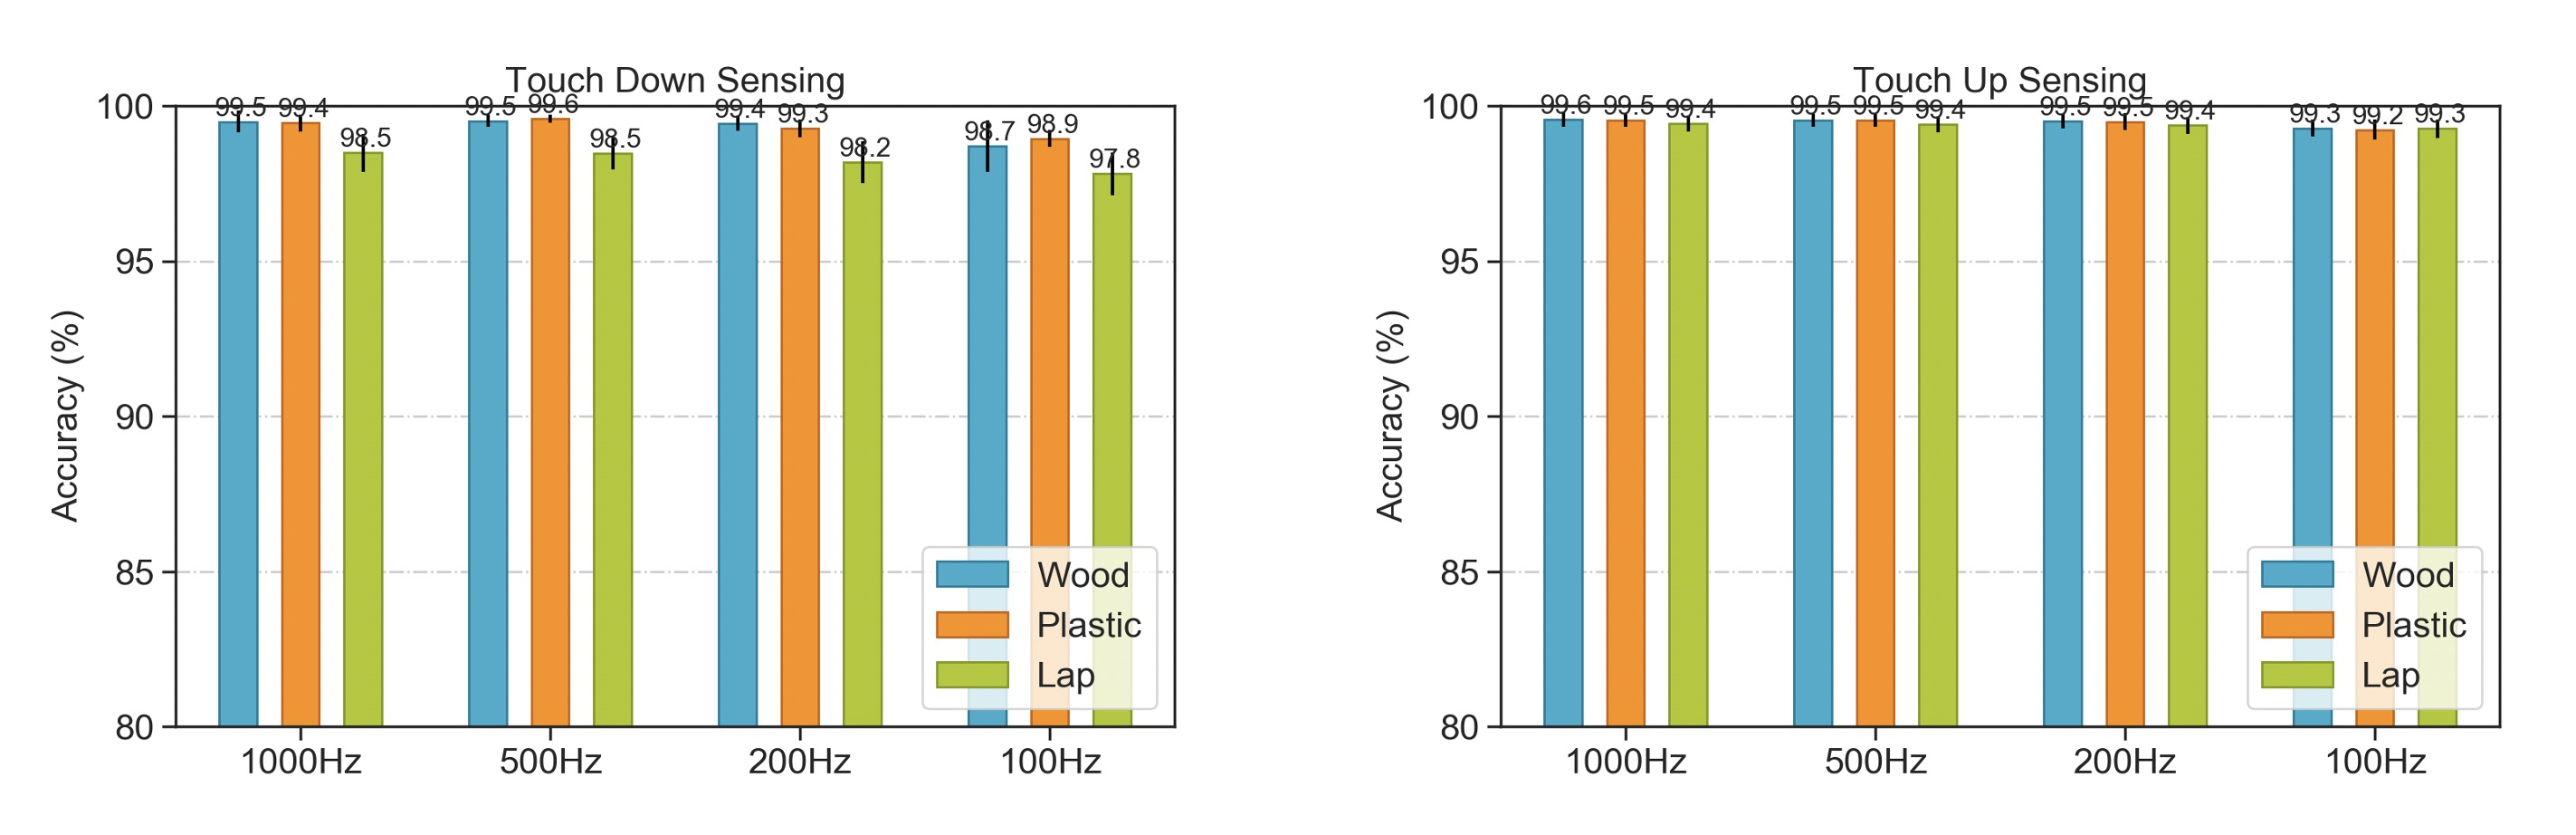
\includegraphics[width=1.0\linewidth]{acc_over_freq.jpg}
	\caption*{如图所示,当采样频率降低时,触摸事件和抬起事件的识别准确率都会受到影响,但总体而言,200赫兹下的识别准确率已经很高。}
	\caption{降采样情况下触摸手势识别的准确率}
	\label{fig:acc_over_freq}
\end{figure}

对于触摸事件识别,双因素重复测量方差分析显示,传感器频率对识别准确率有显著影响($F_{3,33}=16.44,p<.001$)。Bonferroni 校正的后验测试显示以下频率之间存在显著差异:1000Hz-100Hz(p<.001)、500Hz-100Hz(p<.001)、200Hz-100Hz(p<.05)。对于抬起事件识别,频率对性能也有显着影响($F_{3,33}=39.94,p<.001$),Bonferroni 校正的后验测试显示以下频率之间存在显著差异:1000Hz-100Hz(p<.001)、500Hz-100Hz(p<.001)、200Hz-100Hz(p<.001)。结果表明,虽然降低频率的确会影响触摸手势识别的准确率,但是200赫兹以上的传感信号已经能提供较高的识别准确率了。

\section{智能打字指环的解码器设计}

\subsection{实验二:收集打字数据}

本实验的目的是收集被试的打字行为数据,用以设计文本输入单词解码器。在使用智能打字指环输入文本时,用户不能在无源表面上看到键盘布局,相反,用户需要回忆平时打字时每个字母的键位,在桌面上想象一个键盘来打字。本实验通过收集用户打字的数据来确定想象键盘的空间位置参数,实验者也通过这个实验来观察被试的打字行为。

\subsubsection{实验设计和过程}

实验者从校园中招募了12名被试,被试的年龄从19岁到29岁不等,平均年龄为23.67岁,标准差为3.14,其中4名被试为女性。以上被试均为参与过之前的用户实验。在正式实验开始前,有一个简短的熟悉阶段。实验者向被试介绍想象键盘的概念,特别是向被试介绍清楚想象键盘的边界(如图\ref{fig:QwertyRing_teaser}B-E所示)。然后,被试按顺序键入从A到Z的二十六个英文字母,以熟悉自己心中想象键盘中每个按键的位置。通过平移手腕而不是旋转手腕来打字是智能打字指环的用法中禁止的,但时常被被试忽略,因此,实验者在熟悉阶段中会纠正被试平移手腕的问题。熟悉阶段的时长大约为五分钟,实验由五段重复的实验组成。在每段实验中,被试需要誊写十个短句,这些短句是从MacKenzie短句集\cite{mackenzie2003phrase}中随机抽取的。

\begin{figure}[!htbp]
	\centering
	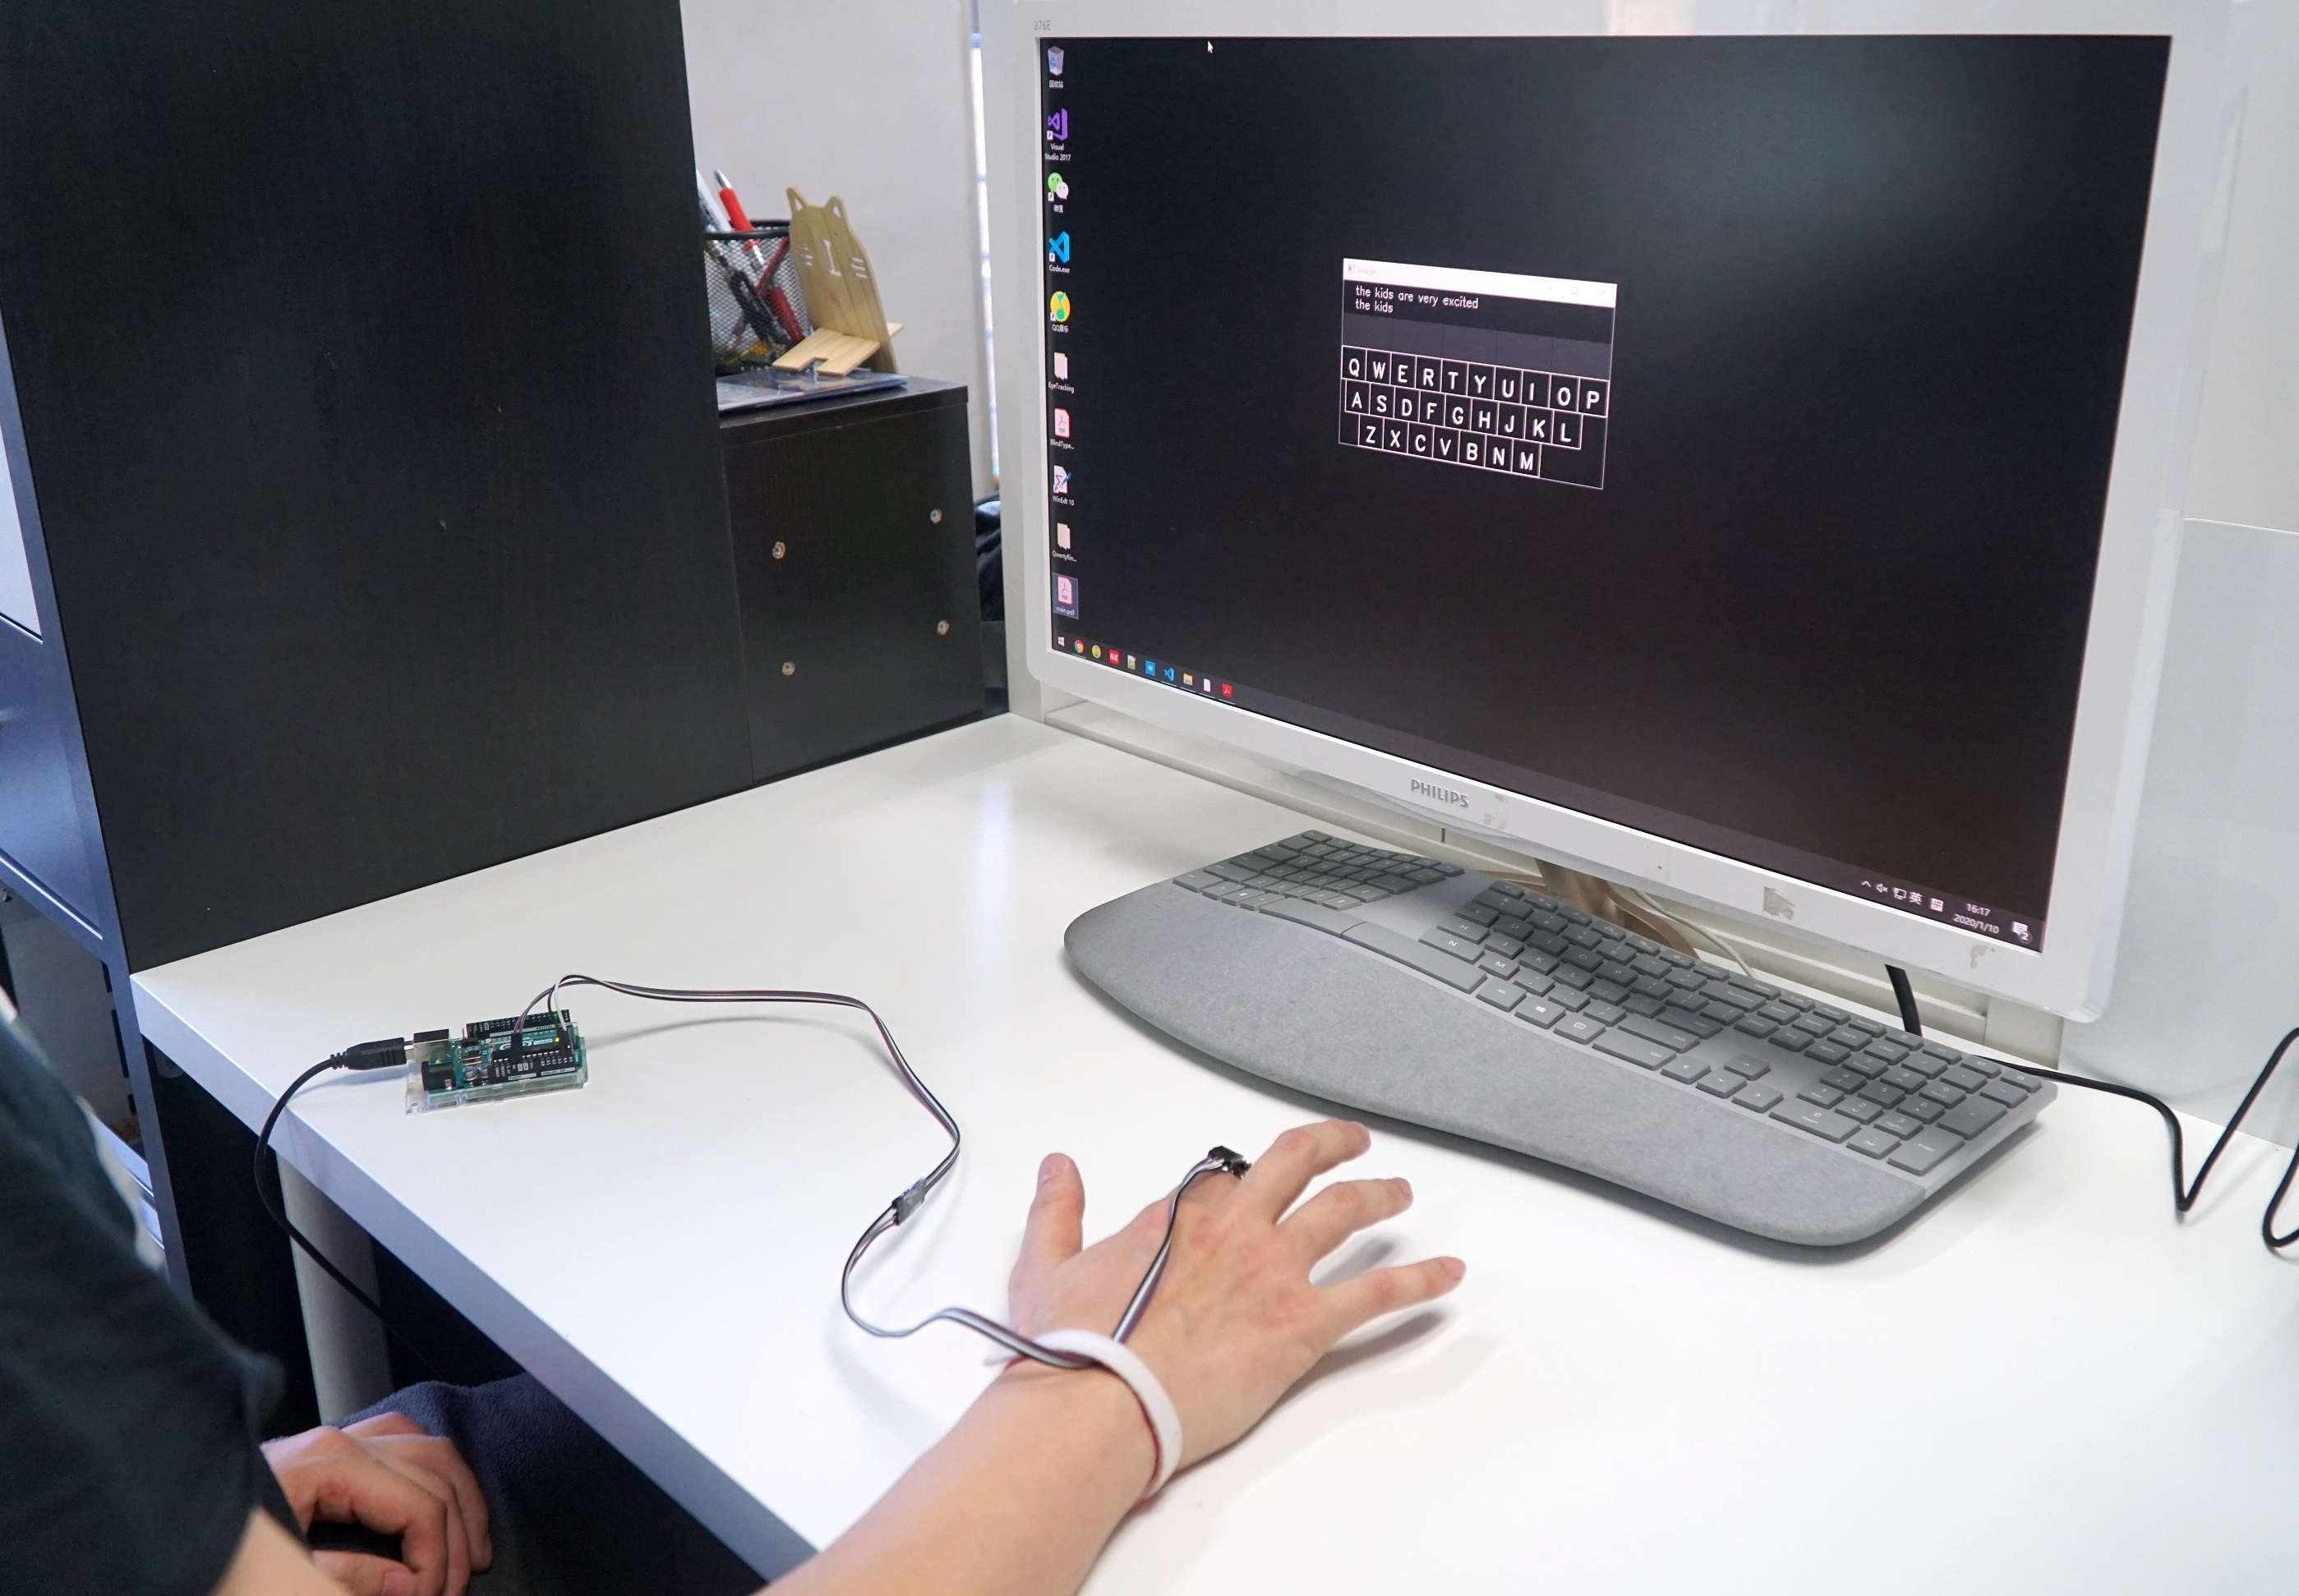
\includegraphics[width=0.8\linewidth]{figures/QwertyRing_config2.jpg}
	\caption*{图中展示了实验二的实验设置,被试佩戴惯性传感指环在一张普通桌子上打字,通过一个显示器接收视觉反馈。}
	\caption{实验二的实验设置}
	\label{fig:QwertyRing_config2}
\end{figure}

如图\ref{fig:QwertyRing_config2}所示,被试坐在可调节的座椅上进行实验。被试可以将椅子调整到最舒适的高度和角度。一台显示器中展示了用户界面,包括二十六键键盘的布局、任务中要求誊写的句子,和已经输入的单词。被试佩戴智能打字指环,在一张普通的桌子上打字,实验者要求被试尽可能又快又准地誊写短句。在实验二中,系统还没有单词解码器,用户不能真的按自己的意愿输入单词:无论被试如何打字,系统都将始终显示正确的字符。但是,如果被试自己主观上发现自己打错了,则应该重做正在输入的短句。之前也有工作\cite{lu2017blindtype, azenkot2012touch, findlater2011typing}采用相同的方法来收集理想的打字行为数据。实验中,被试被要求将视觉注意力集中在显示器上,而不是看着自己的手部。整个实验的时长约为一个小时。

\subsubsection{数据处理}

智能打字指环的基本思想是通过惯性传感指环的方位角来预测用户想要输入的单词。惯性传感器的俯仰角和偏航角对单词解码器来说有用:(1)\textbf{俯仰角(Pitch)}指的是手指指向与水平面的夹角,当用户在想象键盘上点击位于不同行的字母时,惯性传感指环的俯仰角也是不同的;(2)\textbf{偏航角(Yaw)}指的是手指绕竖直轴的旋转角度,当用户在想象键盘上点击位于不同列的字母时,偏航角是不同的。实验者使用Madgwick滤波器\cite{madgwick2010efficient}来获取惯性传感器的俯仰角。然而,惯性传感器所提供信息无法获取绝对的偏航角,实验者通过偏航角上角速度的积分来估计两次点击之间的偏航角增量($\Delta{Yaw}$):

\begin{equation}
	\Delta{Yaw} = \Sigma^{T}_{i=1}G_{zi}\Delta{t_i}
\end{equation}

其中,T是连续两次点击之间的信号帧数,$G_{zi}$是第i帧中惯性传感器角速度的z轴分量,$\Delta{t_i}$是第i帧的持续时长。

接下来,首先形式化本节可能涉及的量。假设实验中,被试们点击字母$u$共计$N_u$次,本文将所有敲击字母$u$时惯性传感指环的俯仰角的集合表示为$P_u=\{{Pitch_u}_i\}^{N_u}_{i=1}$,将偏航角的集合表示为$Y_u=\{{Yaw_u}_i\}^{N_u}_{i=1}$。假设实验中,被试们共有$N_{u,v}$连续点击了$u$和$v$这两个字母,本文使用$\Delta{Y}_{u,v}=\{{\Delta{Yaw_{u ,v}}_i}\}^{N_{u,v}}_{i=1}$来表示它们的偏航角增量的集合。受限于惯性传感器的能力,本实验所收集的数据包括绝对俯仰角$P_u$和相对偏航角$\Delta{Y}_{u,v}$,但不包括绝对偏航角$Y_u$,这是因为,六轴的惯性传感数据不可能还原出绝对偏航角。对于每个被试的$P_u$和$\Delta{Y}_{u,v}$,实验者都剔除了三个标准差以外的极端数据。
 
\subsubsection{实验结果}

同一个用户想要键入同一个字母$u$时,其手指的方位角是类似的。因此,$P_u$和$Y_u$应服从某种概率分布。根据论文BlindType\cite{lu2017blindtype}中所介绍的相对触点模型,$\Delta{Y}_{u,v}$也服从某种概率分布。为了简化计算,实验者假设$P_u$和$\Delta{Y}_{u,v}$都符合二维正态分布,这次文本输入相关工作中常用的假设\cite{lu2017blindtype, yu2017tap}。由于$P_u$和$\Delta{Y}_{u,v}$是由实验直接测得的,实验者拟合了它们的二维正态分布$(\overline{P_u},\sigma{P_u})$和$(\overline{Y_{u,v}},\sigma{Y_{u,v}})$,单词解码器会用到以上两个分布,这将在后续的一节中介绍。然而,$Y_u$不可由实验设备直接测得,实验者间接地通过求解以下最优化问题来估计它的取值,使之最符合实验的观测结果:

\begin{equation}
\begin{cases}
\overline{Y_u} \\
min \sum_{u}\sum_{v}N_{u,v}((\overline{Y_v}-\overline{Y_u})-\overline{\Delta{Y}_{u,v}})^2
\end{cases}
\end{equation}

其中,$\overline{Y_u}$是点云$Y_u$的均值,实验者通过最速下降算法求解上述最优化问题。

\begin{figure}[!htbp]
	\centering
	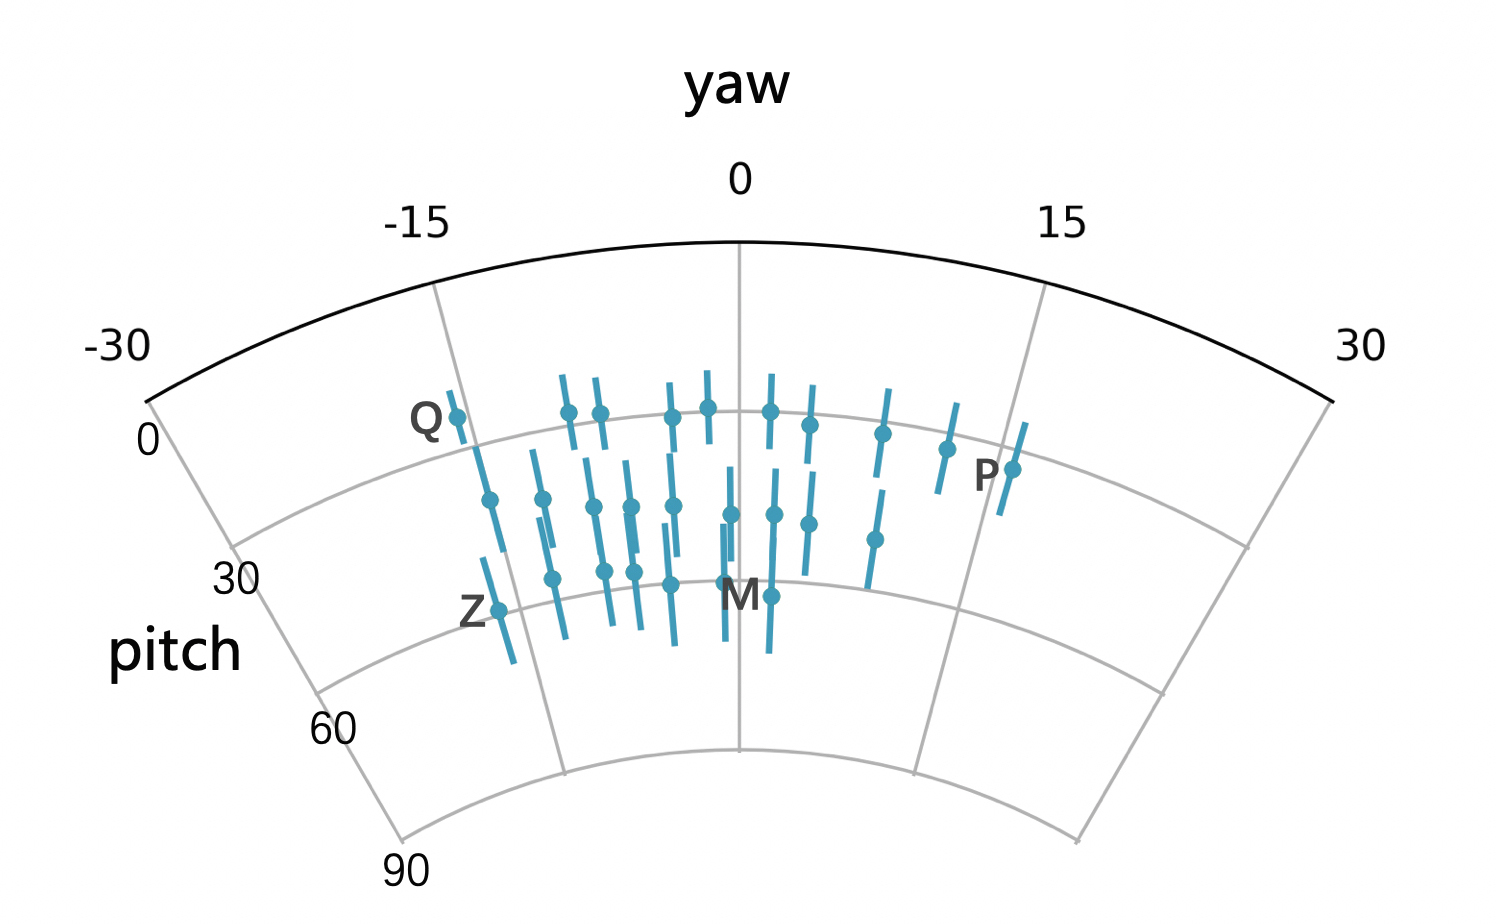
\includegraphics[width=0.8\linewidth]{figures/QwertyRing_point_cloud.jpg}
	\caption*{如图所示是被试们使用智能打字指环打字时,二十六个键位对应的俯仰角和偏航角点云。其中,误差条表示俯仰角的标准差。}
	\caption{平均意义下的触点点云}
	\label{fig:QwertyRing_point_cloud}
\end{figure}

如图\ref{fig:QwertyRing_point_cloud}所示是所有被试平均情况下的二十六键触点点云$(\overline{Y_u},\overline{P_u})$,它反映了平均意义下被试们心中想象键盘的布局。如实验者所期待,惯性传感器的俯仰角和偏航角很好地表征了用户所想输入按键的行号和列号。想象键盘的左边边界在字母Z上,右边边界在字母P上,其偏航角跨度为$32.4^\circ$。想象键盘的上下边界在字母Q和M上,分别对应$24.1^\circ$和$62.6^\circ$俯仰角,其跨度为$38.4^\circ$。

\begin{figure}[!htbp]
	\centering
	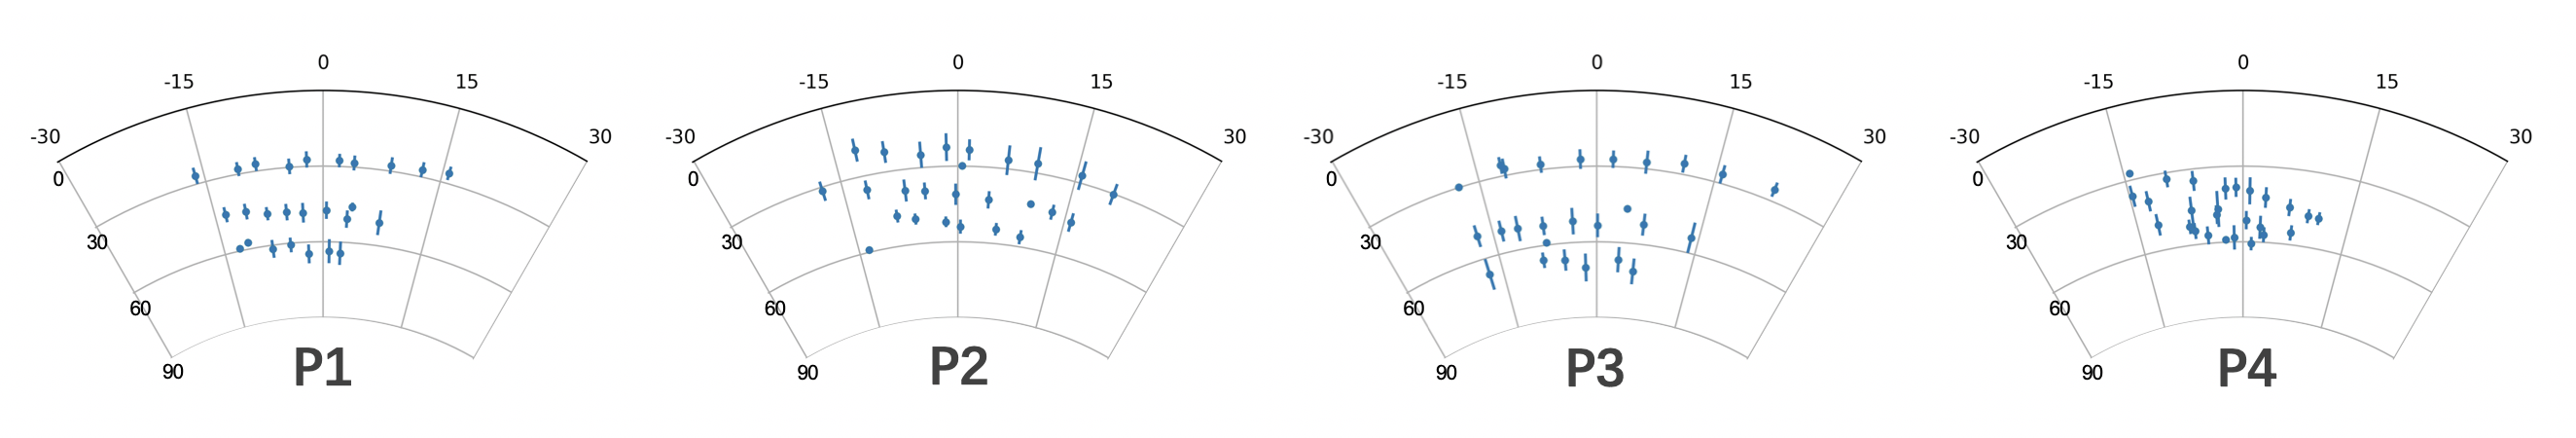
\includegraphics[width=1.0\linewidth]{figures/QwertyRing_pc_over_people.png}
	\caption*{如图所示是四名不同被试的触点点云,误差条表示俯仰角的标准差。}
	\caption{不同被试的触点点云}
	\label{fig:QwertyRing_pc_over_people}
\end{figure}

图\ref{fig:QwertyRing_pc_over_people}展示了四名典型被试的二十六键触点点云,从图中可以看出,被试们心中的想象键盘在大小和形状上都存在较大差异。最大的想象键盘(被试P3)的偏航角跨度和俯仰角跨度为$40.1^\circ \times 45.7^\circ$,而最小的想象键盘(被试P4)为$25.3^\circ \times 33.4^\circ$。被试P1通常以差不多的俯仰角点击位于键盘同一行的按键,也就是说,他的想象键盘是扇形的。被试P2在点击左上角的按键时手指伸得更远,实验者推测,这位被试的想象键盘是一个向左偏的矩形,因此他认为左上角的键是最远的。

\subsection{智能打字指环单词解码器}

智能打字指环单词解码器的工作原理是贝叶斯方法,该方法通过以下公式评估单词$W$作为用户所想单词的概率,然后选出概率最大的五个候选词供用户选择:

\begin{equation}
	P(W|I) \propto P(I|W) \times P(W)
	\label{equ:beyesian}
\end{equation}

其中,$I$是用户输入此单词时的触点序列,每个触点用手指接触交互表面时惯性传感器的偏航角和俯仰角表示。本节将从触点模型$P(I|W)$和语言模型$P(W)$两个方面介绍单词解码器。本节中涉及到的模拟实验评测都基于实验二中收集的数据。

\subsubsection{触点模型}

$P(I|W)$是贝叶斯单词解码器的触点模型部分:

\begin{equation}
	P(I|W) = \prod^{n}_{i=1}P(I_i|W_i)
	\label{equ:beyesian_touch}
\end{equation}

其中,$n$是单词$W$的长度,$W_i$表示单词的第$i$个字母,$I_i$表示用户输入该单词时的第$i$次触点。在类似的工作中,研究者一般认为触点服从二维高斯分布\cite{goodman2002language, azenkot2012touch},这是绝对触点模型;同时,也有研究者指出,连续两次触点之间的向量也服从二维高斯分布\cite{lu2017blindtype},这是相对触点模型。在本节所介绍的单词解码器中,受限于惯性传感指环的识别能力,实验者假设绝对触点模型适用于触点的俯仰角,而相对触点模型适用于偏航角。也就是说,触点俯仰角集合$P_u$和相邻两次触点之间的偏航角增量集合$\Delta{Y_{u,v}}$都服从二维正态分布,因此,$P(I|W)$可以表示为:

\begin{equation}
	P(I|W) = \prod^{n}_{i=1}P(Pitch_i|W_i)\prod^{n-1}_{i=1}P(\Delta{Yaw}_{i,i+1}|W_{i,i+1})
	\label{equ:beyesian_relative}
\end{equation}

其中,$Pitch_i$是用户输入字母$W_i$时惯性传感指环的俯仰角,$\Delta{Yaw}_{i,i+1}$是用户在输入字母$W_i$和$W_{i+1}$的时间段内手指的偏航角增量。单词解码器可以利用实验二中整理出来的分布$P_{W_i}$和$Y_{W_i,W_{i+1}}$来计算上述公式中的值$P(Pitch_i|W_i)$和$P(\Delta{Yaw}_{i,i+1}|W_{i,i+1})$。

\subsubsection{语言模型}

\begin{figure}[!htbp]
	\centering
	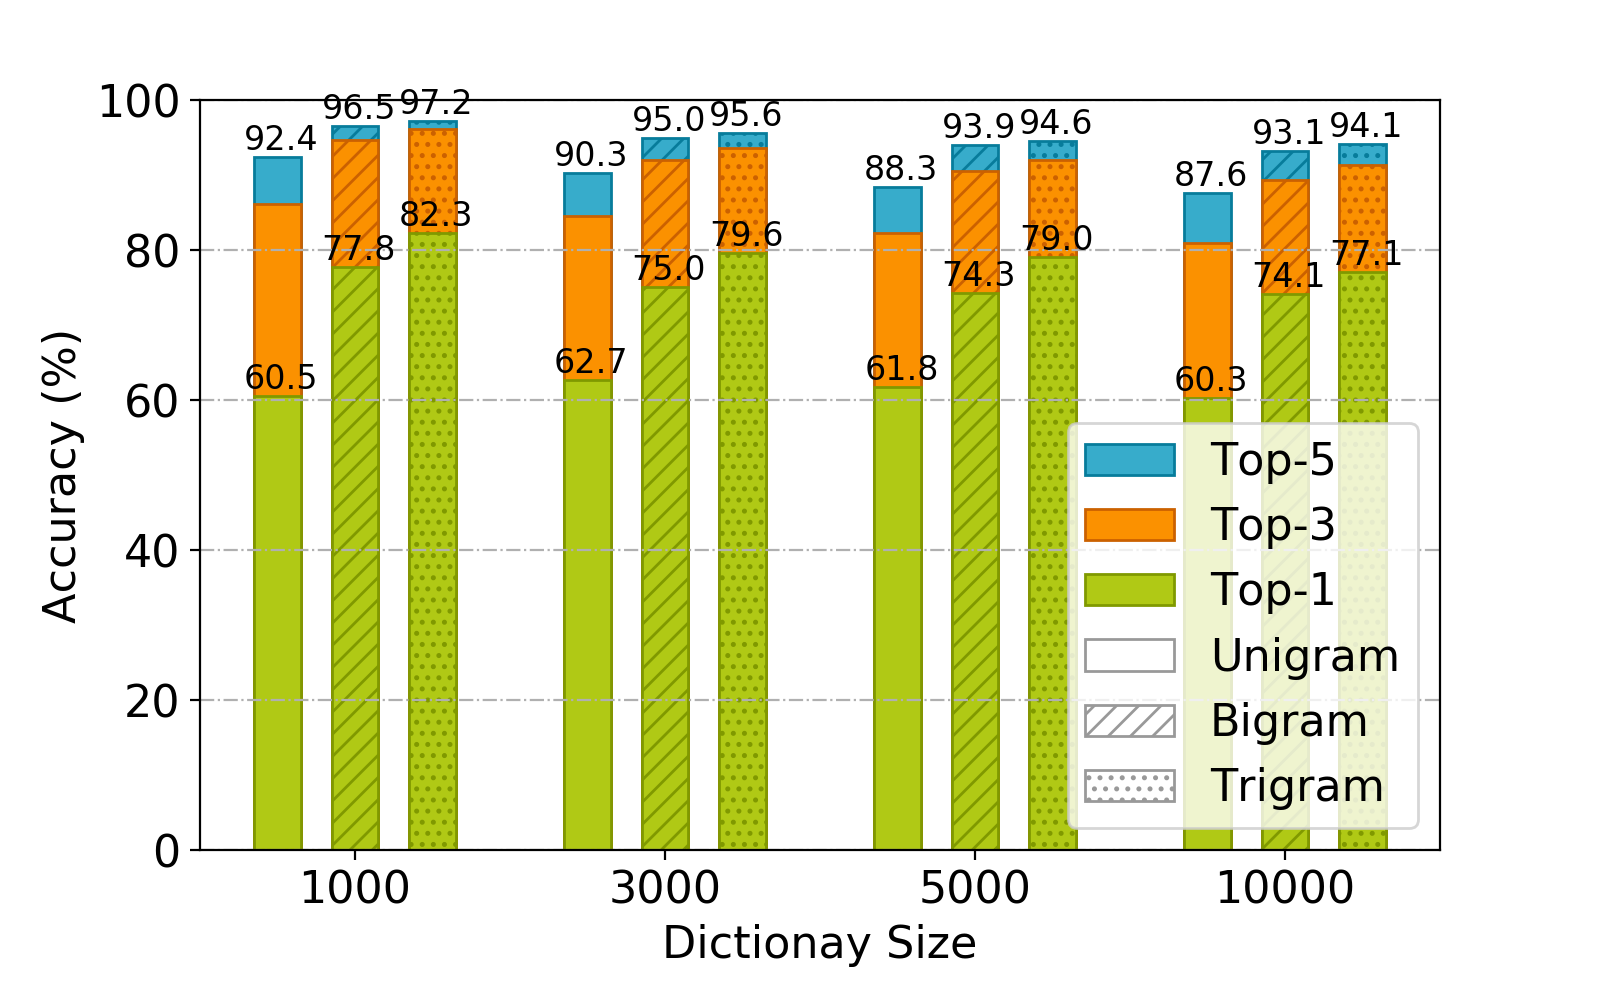
\includegraphics[width=0.8\linewidth]{figures/QwertyRing_language_model.png}
	\caption*{如图所示是不同语言模型下,解码器在不同词库大小下的单词预测准确率。}
	\caption{不同语言模型下解码器的预测准确率}
	\label{fig:QwertyRing_language_model}
\end{figure}

$P(W)$是单词解码器中的语言模型部分。实验者通过模拟实验测试了单元、双元、三元语言模型的性能\cite{ide2008american}。单元语言模型通过大型预料库中每个单词的出现频次来估计每个单词出现的概率$P(W)$,双元语言模型中的$P(W)$是将前一个已输入单词作为前提条件时下个单词为$W$的概率,三元语言模型则是考虑前两个已输入的单词。如图\ref{fig:QwertyRing_language_model}所示是应用不同语言模型时,解码器在不同词库大小下的单词预测准确率。其中,Top-1、Top-3、Top-5准确率指的是用户所想单词出现在候选词列表第一位、前三位和前五位的概率。

二元重复测量方差分析显示,语言模型对解码器的Top-1准确率有显著性影响($F_{2,22}=86.53,p<.001$)。三元语言模型显著优于双元语言模型($p<.001$)和单元语言模型($p<.001$),在词库大小为5000的情况下它的Top-1准确率达到79.0\%,Top-5准确率达到94.6\%。也就是说,当用户使用智能打字指环输入一篇词汇量在5000个单词以内的文章时,单词解码器将用户手指敲击桌面的信号直接转化为他想要的单词的概率是79.0\%,用户能通过选词功能选中所需单词的概率是94.6\%。由于三元语言模型的表现是最好的,在本章的剩余内容中都默认使用三元语言模型。方差分析还显示,词库大小对解码器的Top-1准确率的影响只是一个趋势($F_{3,33}=2.41,p=.085$),还不是显著的。这是因为在本实验的测试短句中,以及在日常打字过程中,出现低频词汇的概率是很低的。

\subsubsection{用户个性化}

实验二曾发现被试的打字行为差异很大,这启发实验者研究解码器是否应该针对用户个性化做出优化。本章将\textbf{通用化模型}定义为通过实验二所有被试的数据训练得到的单词解码器;而\textbf{个性化模型}是在通用化模型的基础上,不断通过特定用户输入数据更新自身参数的单词解码器。在实际应用场景中,所有用户刚开始只能使用通用化模型作为智能打字指环的单词解码器,个性化模型不断收集用户的打字数据,并试图在数据量足够大的时候更新某些按键的触点分布$P_u$或$\Delta{Y}_{u,v}$。更具体地,当特定用户个人的触点集合$P_u$或$\Delta{Y}_{u,v}$的大小大于等于8时,个性化的单词解码器就会根据触点集合重新计算其分布,其中,阈值8是模拟实验得到的最佳阈值。

\begin{figure}[!htbp]
	\centering
	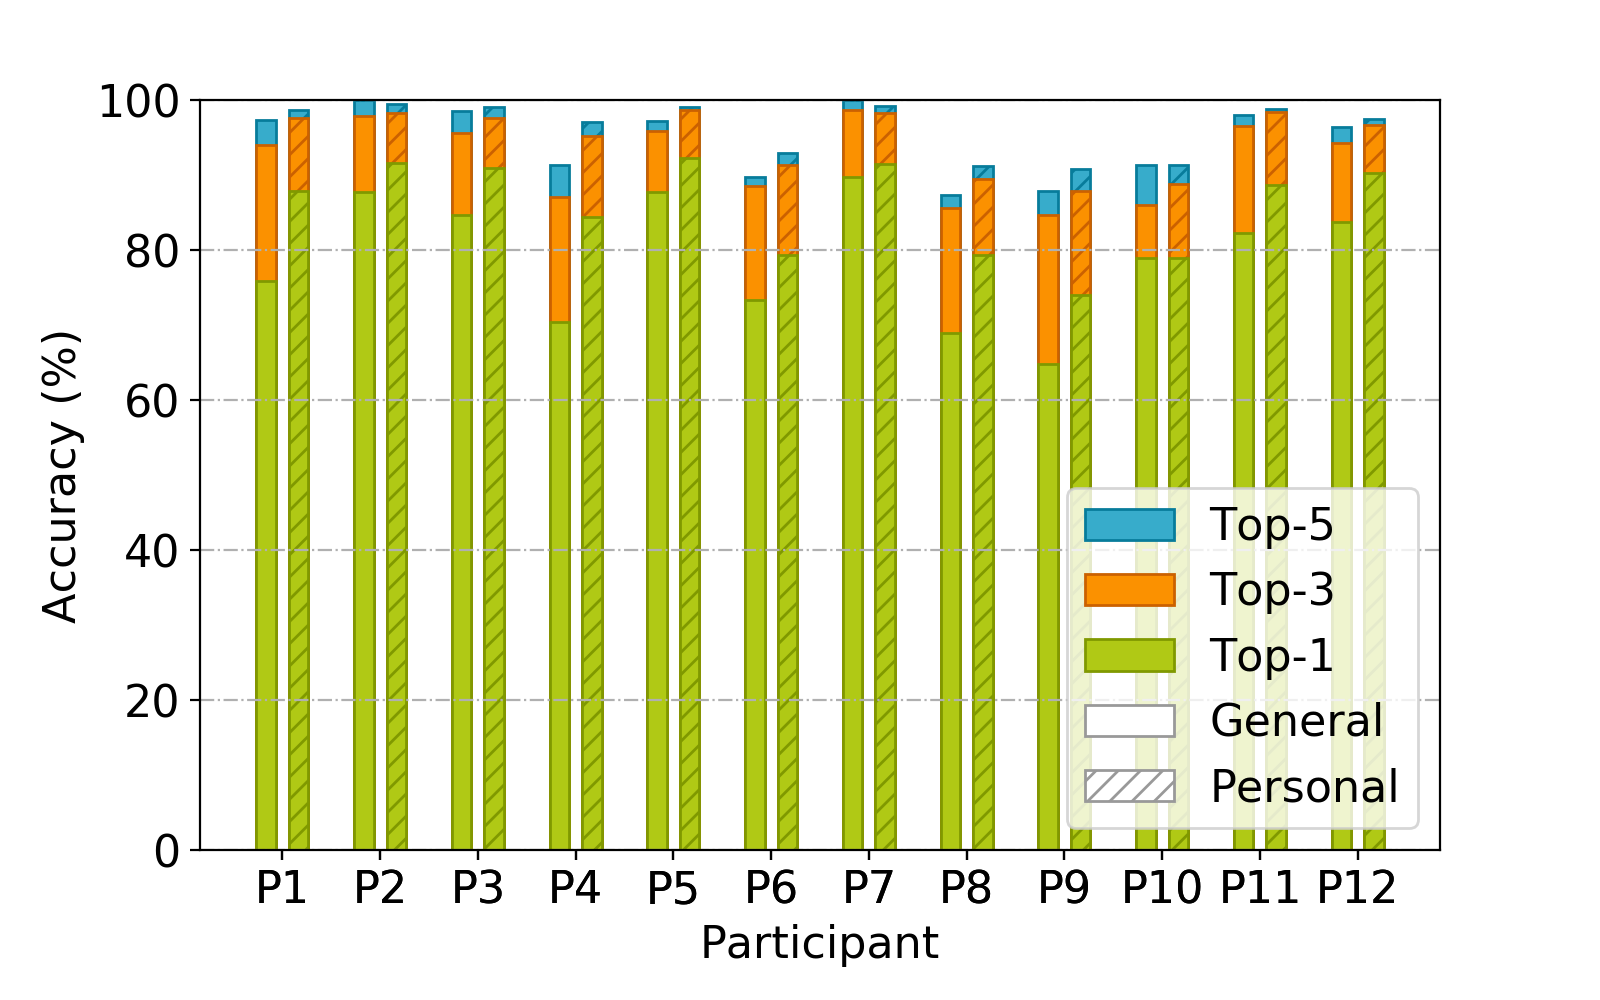
\includegraphics[width=0.8\linewidth]{figures/general_vs_personal.png}
	\caption*{图中展示了通用化模型和个性化模型在不同用户的数据上的预测准确率。}
	\caption{通用化模型和个性化模型的预测准确率}
	\label{fig:general_vs_personal}
\end{figure}

图\ref{fig:general_vs_personal}展示了通用化模型和个性化模型的准确率对比。实验者通过五折交叉验证来评测个性化模型的性能,即将实验二中每个人的四段实验数据(40句话)作为训练集,将一段实验数据(10句话)作为测试集。从图中可以看出,个性化的单词解码器的准确率更高。下一个实验将通过正式的用户实验来进一步评测智能打字指环的性能,同时比较通用化模型和个性化模型。

\section{智能打字指环的评测}

\subsection{实验三:智能打字指环的评测实验}

实验三是用于评测的用户实验,有两个目的:一是评测基于惯性传感指环的无源表面文本输入技术(智能打字指环)的打字速度和学习曲线;二是对比上一节所述的通用化模型和个性化模型。

\subsubsection{实验设计和过程}

本实验为期五天,采用组间实验设计来对比通用化模型和个性化模型。实验者从校园中招募了16名被试参与实验,被试的年龄从20岁到27岁不等,平均年龄为22.86岁,方差为2.09,其中有6名女性被试。被试们没有参与过之前的任何用户实验。在每一天的实验中,被试都会誊写30句话,这30句话是从MacKenzie短句库\cite{mackenzie2003phrase}中随机抽取的。

本实验的设置和实验二相似(如图\ref{fig:QwertyRing_config2})。被试坐在可调节的桌椅上,将惯性传感指环佩戴在食指第二骨节上,在一张普通的桌子上输入文本。被试们通过一台显示器接收视觉反馈。实验者要求被试尽可能又快又准地完成文本输入任务,在实验中,被试被要求将视线集中在屏幕上,而不要过多地关注自己的手部。与实验二不同的是,本实验已经应用了智能打字指环文本输入技术,被试需要真正地去打字,单词打错了要删除后重打,而不会像在实验二中一样无论怎样输入都显示正确的字母。

在第一天的实验当中,所有用户都使用基于通用化模型的单词解码器进行实验。通用化模型是由实验二中所有用户的实验数据拟合而成的。从第二天开始,我们将被试分为两组,每组都有八名被试。两组被试的平均年龄分别是22.50岁(SD=1.77)和23.25岁(SD = 2.55),他们两组人在第一天实验中的平均打字速度是尽可能接近的。具体而言,实验者写了一个分组程序,随机将16名被试分组1000次,选取两组人平均打字速度最接近的一种分组方法来实际执行。第一组被试在后续四天的实验中继续使用通用化模型;第二组被试则在后续四天实验中使用个性化模型。对于使用个性化模型进行实验的每一名被试,实验者都会在每天的实验开始前,用该被试已有数据重新拟合个性化的单词解码器。

在第一天的正式实验之前,有一个简短的热身阶段。研究者向被试介绍想象键盘的概念。在实验者的指导下,被试从A到Z点击字母各两次以熟悉想象键盘。然后,被试会尝试输入五句话。整个热身阶段的时长大约为十分钟。在每天的正式实验中,被试分三段实验来誊写30句话,在每两段实验之间休息五分钟的时间。每天实验的时长为一个半小时,五天实验的总时长为七个半小时。

\subsection{智能打字指环的评测结果}

实验者使用混合方差分析来评估组间因素(解码器模型)和组内因素(实验天数)对打字速度、未纠正错误率(UER)和已纠正错误率(CER)的显著性影响。由于UER和CER不服从正态分布,实验者在方差分析之前使用对齐秩变换算法\cite{2011-Aligned}校正数据。如果有任何独立变量或组合对实验结果有显著性影响(p<.05),实验者采用Bonferroni校正后的后验测试来做成对比较。

\subsubsection{打字速度}

本实验对打字速度的测量单位是每分钟输入的英文单词数(WPM)\cite{arif2009analysis},计算公式如下:

\begin{equation}
	WPM = \frac{|S|-1}{T} \times 60 \times \frac{1}{5}
\end{equation}

其中,$|S|$是所誊写句子的字符长度(包括空格),$T$ 用户完成誊写的时长。

\begin{figure}[!htbp]
	\centering
	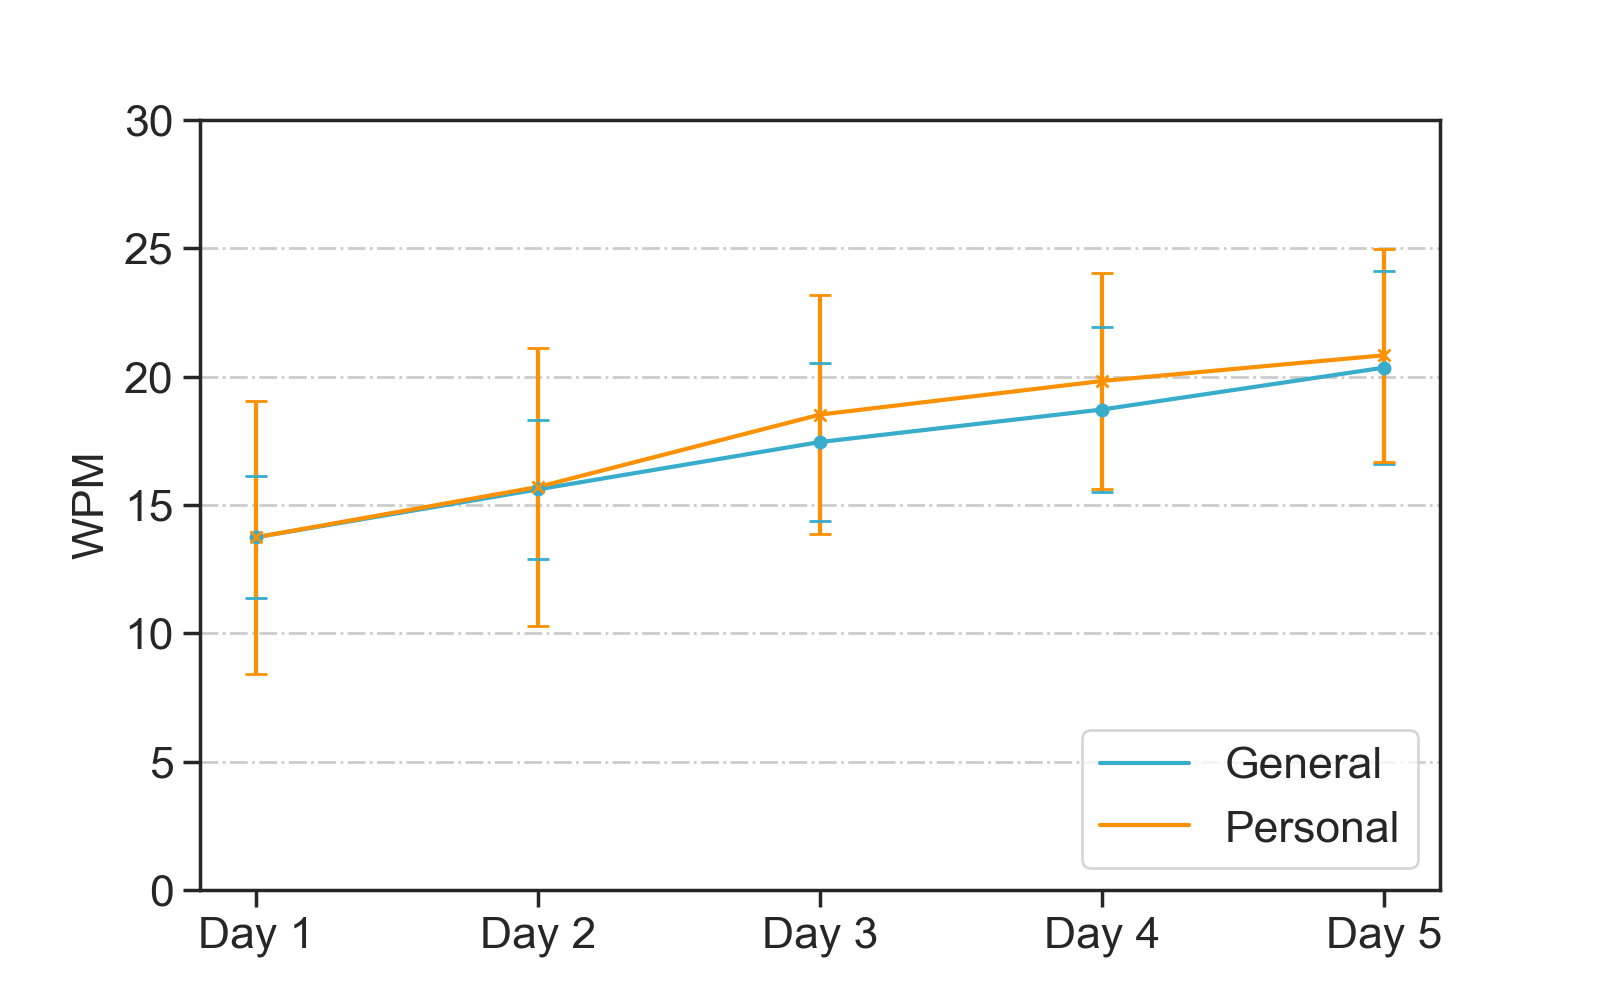
\includegraphics[width=0.8\linewidth]{figures/QwertyRing_wpm.png}
	\caption*{图中展示了被试采用通用化模型或个性化模型时的打字速度随实验天数增加而增长的曲线。}
	\caption{打字速度}
	\label{fig:QwertyRing_wpm}
\end{figure}

如图\ref{fig:QwertyRing_wpm}所示是五天实验中被试打字速度的变化。通用化模型下被试第一天的打字速度为13.75 WPM(SD=2.65),第五天的打字速度为20.83 WPM(SD=4.20)。个性化模型下被试第一天的打字速度为13.74 WPM(SD=5.33),;第五天的打字速度为20.83 WPM(SD=4.14)。模型对打字速度没有显著性影响($F_{1,14}=0.09,p=0.77$)。实验天数对通用化模型下的打字速度($F_{4,28}=27.00,p<.001$)和个性化模型下的打字速度($F_{4,28}=41.17,p<.001$)都有显著性影响。对于通用化模型,后验测试显示以下实验天数之间存在显著差异:1-3(p<.05)、1-4(p<.005)、1-5(p<.005)、2-4(p<.05)、2-5(p<.05)、3-5(p<.05)和4-5(p<.05)。对于个性化模型,以下实验天数之间存在显著性差异:1-3(p<.01)、1-4(p<.005)、1-5(p<.001)、2-3(p<.005)、2-4(p<.005)、2-5(p<.005)、3-5(p<.05)。模型和实验天数之间不存在显著的交互作用($F_{4,56}=0.60,p=0.66$)。图中的学习曲线在最后一天中并未收敛,因此本实验不反映该技术的专家级打字速度。

\subsubsection{打字错误率}

两种指标被用于评测本文本输入法的错误率:(1)未纠正错误率(UER)——遗留在所誊写文本中的错误,UER等于未经纠正的单词数量除以所誊写句子的单词数量;(2)已纠正错误率(CER)——那些在打字过程中被纠正(例如通过删除)的错误,CER等于被纠正的单词数量除以所誊写句子的单词数量。

\begin{figure}[!htbp]
	\centering
	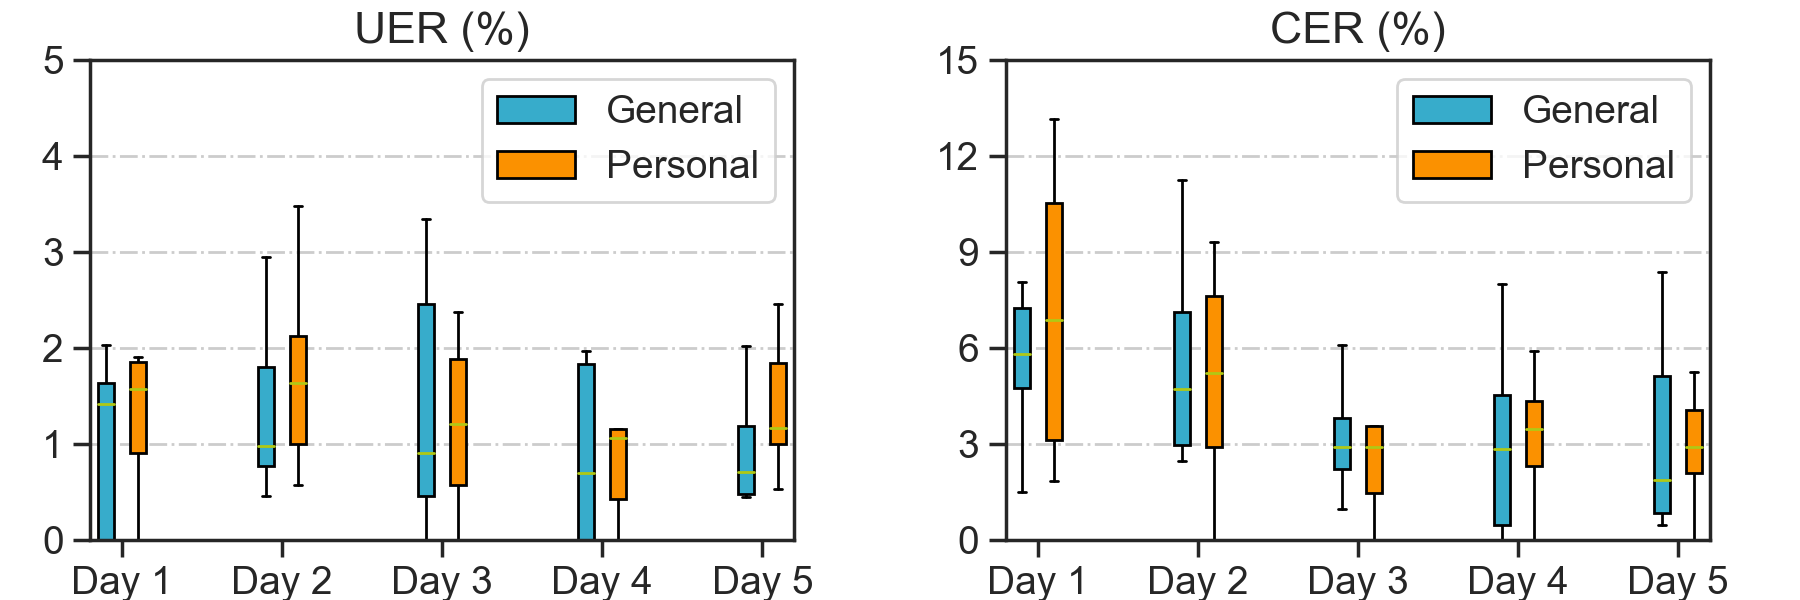
\includegraphics[width=1.0\linewidth]{figures/QwertyRing_uer_cer.png}
	\caption*{图中展示了被试采用通用化模型或个性化模型时的打字错误率随实验天数而变化的箱型图。}
	\caption{错误率}
	\label{fig:QwertyRing_uer_cer}
\end{figure}

如图\ref{fig:QwertyRing_uer_cer}所示是五天实验中UER和CER的变化。模型和实验天数都对UER没有显著性影响。通用化模型下平均UER为1.17\%(SD = 1.02\%),个性化模型下平均UER为1.50\%(1.40\%)。模型对CER没有显著性影响,但实验天数对CER存在显著性影响($F_{4,56}=6.84,p<.005$)。后验测试表明以下实验天数之间CER存在显著性差异:1-3(p<.005)、1-4(p<.05)、1-5(p<.005)、2-3(p<.05)和2-5(p<.05)。在第五天的实验中,通用化模型下平均CER为3.22\%(SD=2.92\%),个性化模型下平均CER为2.92\%(SD=1.65\%),也就是说,被试每输入30个英文单词才需要纠错一次。

\subsubsection{解码器准确率}

\begin{figure}[!htbp]
	\centering
	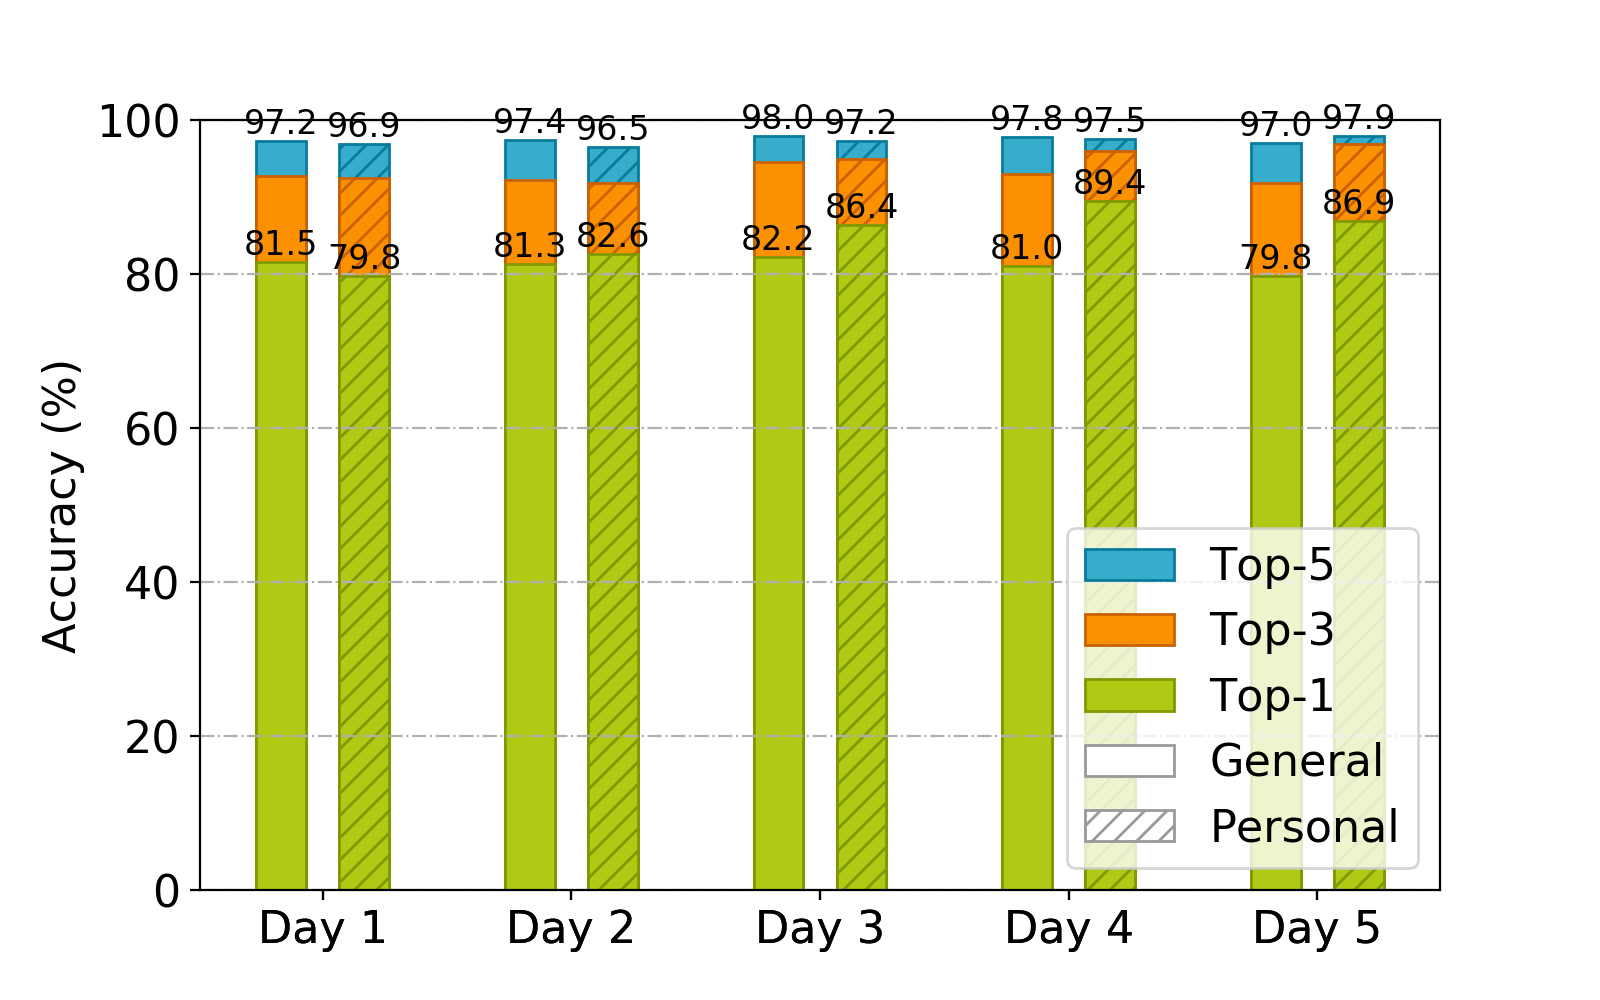
\includegraphics[width=0.8\linewidth]{figures/QwertyRing_predict_acc.png}
	\caption*{图中展示了两种模型下单词解码器的准确率随实验天数而变化的柱状图,准确率指标包括Top-1、Top-3和Top-5准确率。}
	\caption{单词解码器的准确率}
	\label{fig:QwertyRing_predict_acc}
\end{figure}

如图\ref{fig:QwertyRing_predict_acc}所示是通用化单词解码器和个性化单词解码器的准确率随实验天数而变化的柱状图。准确率指标包括Top-1、Top-3和Top-5准确率,其中Top-N准确率指的是被试所需单词出现在候选词列表前N位的概率。混合方差分析显示模型对Top-1、Top-3和Top-5准确率都没有显著性影响。实验天数对通用化模型下的单词解码准确率没有显著性影响,但对个性化模型下的Top-1准确率存在显著性影响($F_{4,28}=3.45,p<.05$)。结果说明,个性化单词解码器会随着用户的使用而自我改进。混合方差分析显示,从第三天开始,个性化模型的解码准确率就存在超过通用化模型的趋势($F_{1,14}=3.22,p=0.09$)。

\subsubsection{时间构成}

为了深入探讨本技术的用户打字效率问题,实验者将被试的文本输入耗时拆分成三个构成部分:键入时间、选词时间和停顿时间。键入时间指的是被试点击单词各个字母所用的时间,是从被试点击单词首字母到点击单词尾字母之间的时间。选词时间是被试从候选词列表中选中所需单词的时间。停顿时间是从完成一个单词的选词到输入下一个单词首字母所需的时间。上述时间指的都是每输入一个英文单词所消耗的时间。

\begin{figure}[!htbp]
	\centering
	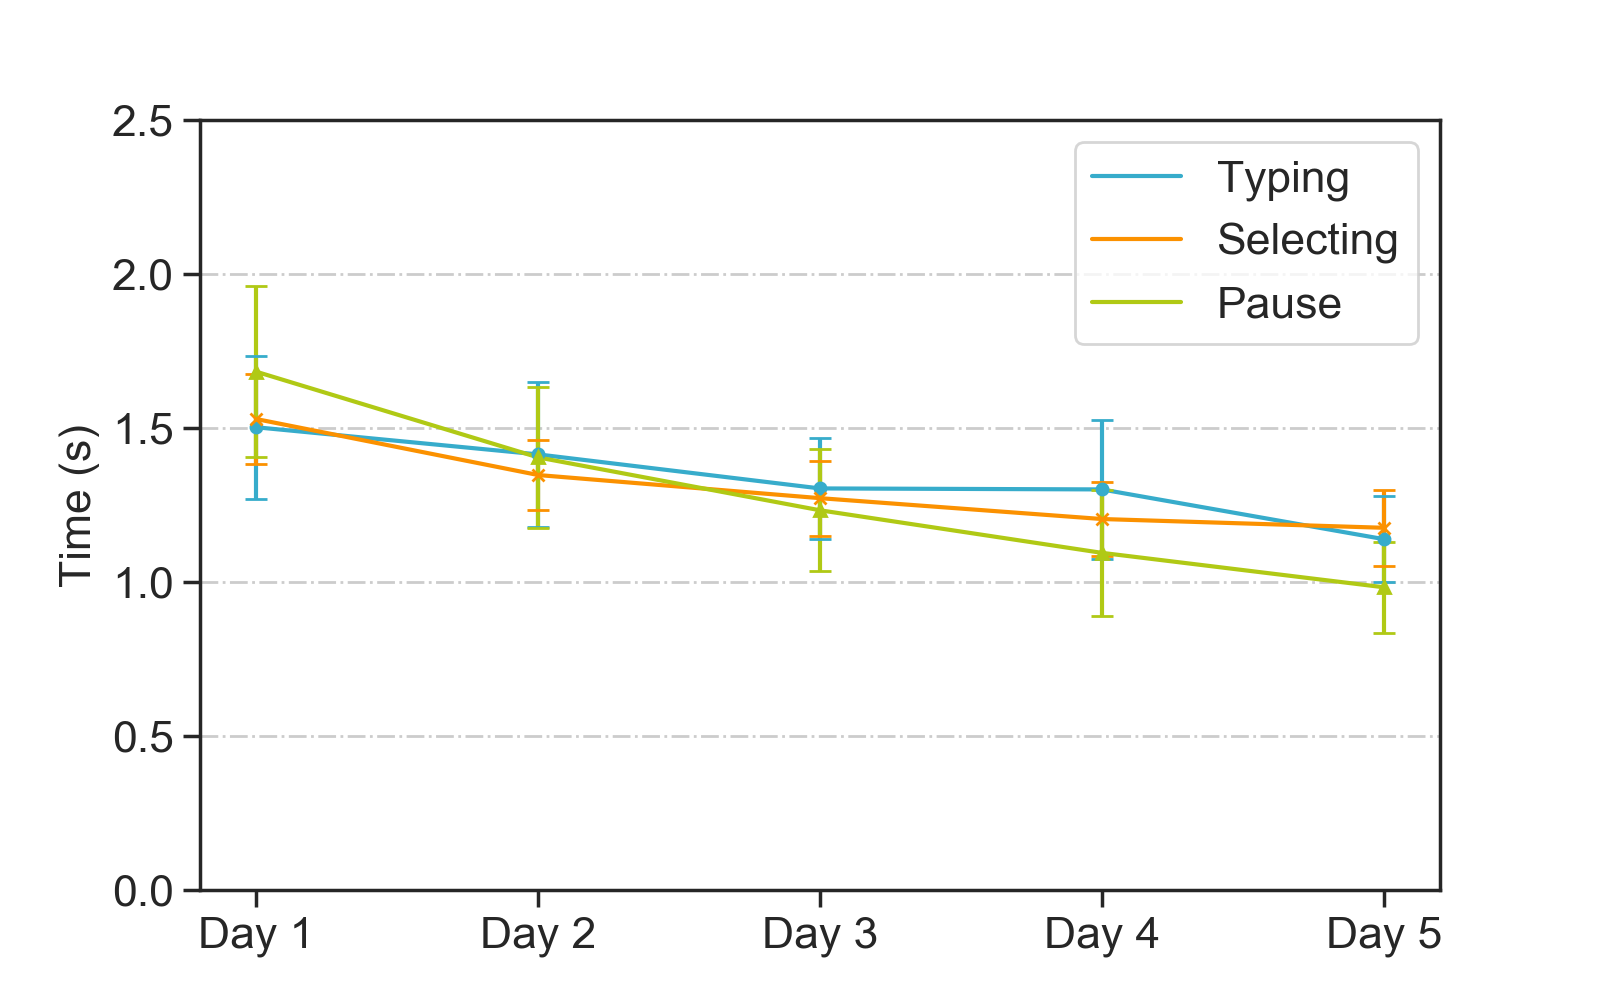
\includegraphics[width=0.8\linewidth]{figures/QwertyRing_time_component.png}
	\caption*{图中展示了被试每输入一个英文单词时各个动作所消耗的时间,误差条表示95\%置信区间。}
	\caption{文本输入时间构成}
	\label{fig:QwertyRing_time_component}
\end{figure}

如图\ref{fig:QwertyRing_time_component}所示是文本输入时间构成随着实验天数变化的曲线。方差分析显示,实验天数对键入时间($F_{4,52}=8.01,p<.001$)、选词时间($F_{4,52}=24.80,p<.001$)和停留时间($F_{4,52}=18.86,p<.001$)都有显著性影响。模型对上述时间构成都没有显著性影响。结果说明,被试在不断打字的过程中学会了更快速地键入字母和选中单词,同时不牺牲选词的准确率。

\begin{figure}[!htbp]
	\centering
	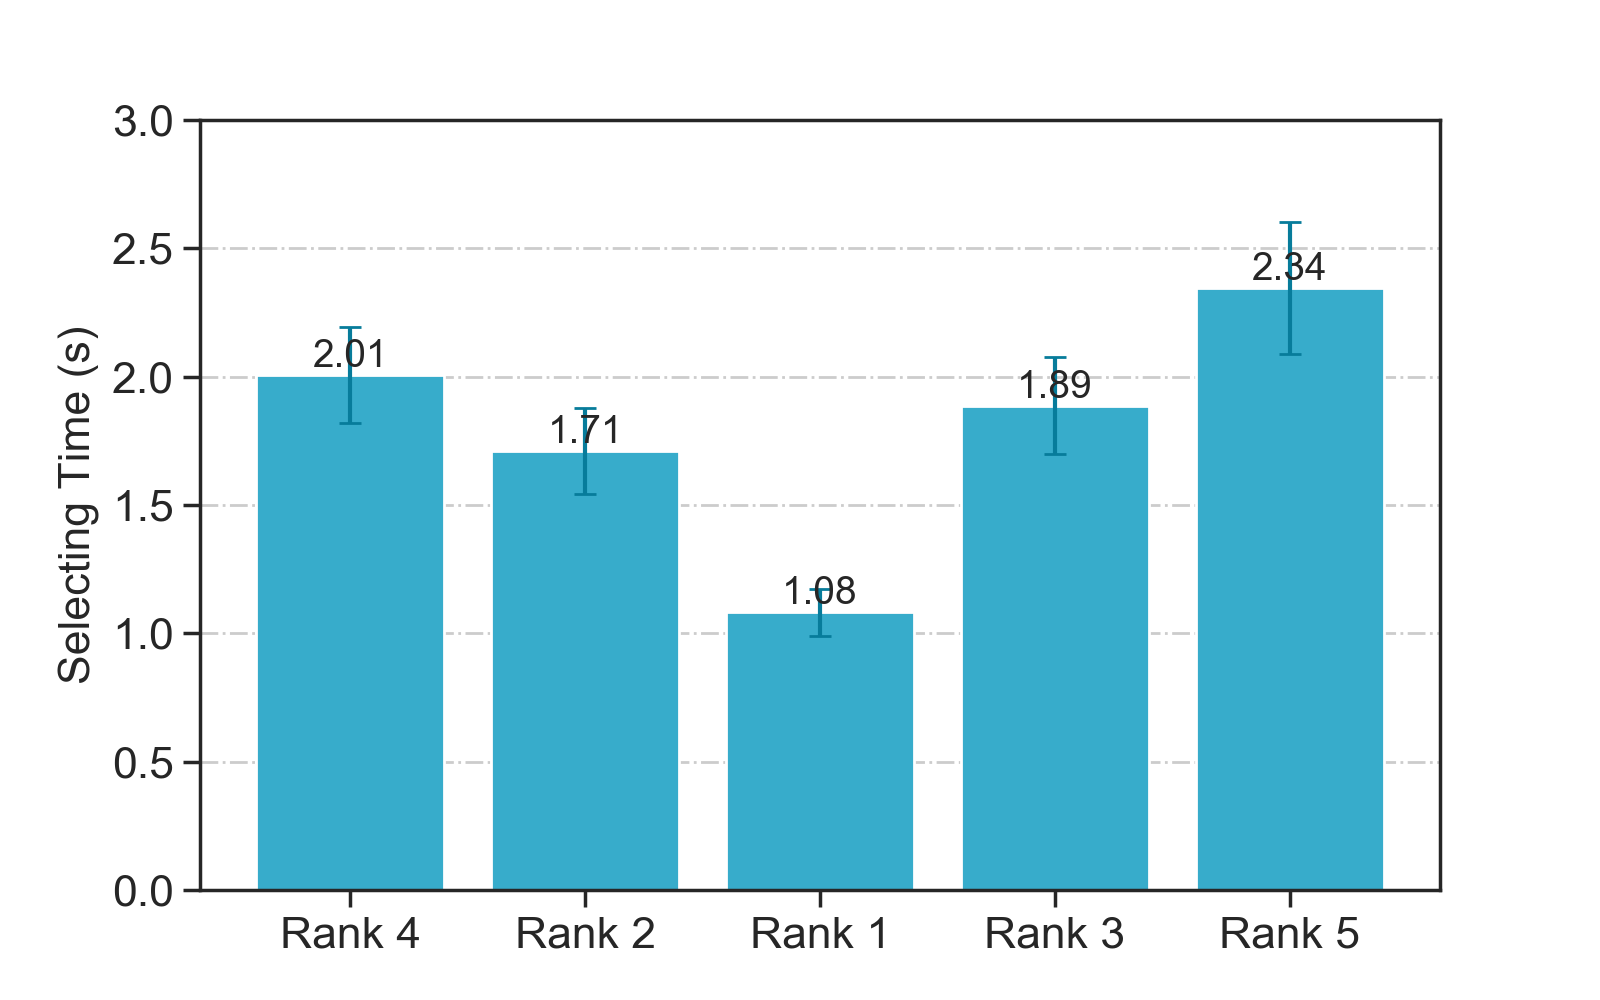
\includegraphics[width=0.8\linewidth]{figures/QwertyRing_selecting_time.png}
	\caption*{图中展示了被试在选中候选词列表中不同单词时的选词时间,误差条表示95\%置信区间。}
	\caption{选词时间}
	\label{fig:QwertyRing_selecting_time}
\end{figure}

图\ref{fig:QwertyRing_selecting_time}进一步探讨了被试所需单词出现在候选词列表不同排位上时被试的平均选词时间。图中从左到右柱子和候选词列表中从左到右单词的顺序相对应,分别对应单词解码排名为第4、第2、第1、第3、第5的单词。从图中可以看出,被试选择排名第一的单词所需的时间是最短的,这是因为在选词开始时,指针已经在该候选词上了。对于排名为2到5名的候选词,实验者发现有两个因素影响了被试的选词时间。第一个影响因素是该候选词距离中央候选词的距离($F_{1,15}=69.47,p<.001$)。第二个影响因素是该候选词位于中央候选词的左侧还是右侧($F_{1,15}=39.76,p<.001$),被试选择左侧候选词比选择右侧候选词更快,这是人的手腕在左右旋转的限制上存在不对称性导致的\cite{grandjean1997fitting}。以上结果说明,在智能打字指环候选词区域的交互设计中,将排名第1的候选词放在中央, 将排第2、第4名候选词放在左侧,第3、第5名候选词放在右侧,是十分科学的。

\subsubsection{主观评分和反馈}

在第一天和第五天的实验结束后,被试都通过一张七级李克特量表对使用本技术时的主观速度、主观准确率、疲劳程度和偏好程度打分(1分-最差;7分最好)。在第一天中,各项主观评价的分数就已经达到了可接受的程度,而且这些分数在第五天的时候得到了提高。对于通用化模型,Wilcoxon Signed-Rank测试表明,主观打字速度($Z=-2.56, p<.05$)和偏好程度($Z=-2.07, p<.05$)在五天的使用过程中得到了改进。对于个性化模型,主观打字速度($Z=-2.21, p<.05$)、主观打字准确率($Z=-2.41, p<.05$)和偏好程度($Z=-2.41, p<.05$)在五天的使用过程中得到了改进。模型对所有主观评分都没有显著性影响。

\begin{figure}[!htbp]
	\centering
	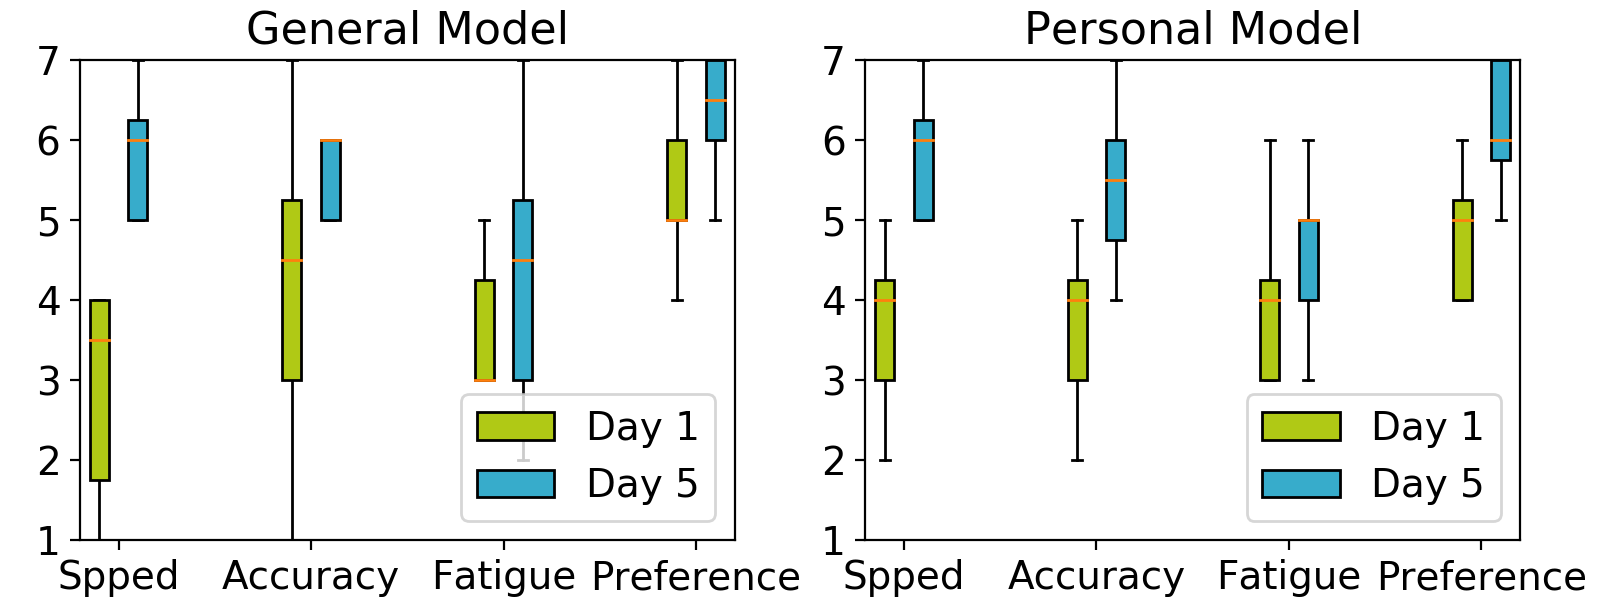
\includegraphics[width=1.0\linewidth]{figures/QwertyRing_subjective.png}
	\caption*{图中展示了通用化模型和个性化模型下,实验第一天和第五天中,各项主观评价指标的分数。}
	\caption{主观评分(1分最差,7分最好)}
	\label{fig:QwertyRing_subjective}
\end{figure}

有两名被试在第一天的实验当中汇报他们在打字20分钟后感到疲劳,从第二天开始他们的疲劳感有所消退。实验观测发现,这两名被试心中的想象键盘布局太大了,这导致了疲劳的问题。当他们逐渐意识到想象键盘实际上可以小一些,并不影响打字的准确率时,他们感受到的疲劳程度就降低了。打字速度最快的被试第一天的打字速度就达到19.37 WPM,第五天时达到29.12 WPM,他从第一天开始就严格遵循了实验者的指导。打字速度最慢的被试第一天打字速度为7.54 WPM,第五天时为16.67 WPM。这名被试犯了平移手腕的错误,这是智能打字指环使用方法中禁止的,会导致惯性传感指环很难获取表征用户点击位置的有效信息。然而在接下来的实验中,这名被试逐渐克服了困难,并且达到了一个可以接受的打字速度。

\subsection{与手机打字速度进行比较}

实验者组织了一场额外的用户实验来评测智能手机上食指打字的速度,实验的目的是比较智能打字指环和常用文本输入技术。实验者选择智能手机上的食指打字为基线技术,这是因为(1)智能手机上的文本输入是常用的,为被试所熟悉;(2)因为智能打字指环中被试使用食指输入文本,本实验也采用食指打字的方案。实验三中的16名被试参与了本实验,实验任务是分三段实验誊写30句话,每两段实验之间休息1分钟的时间。实验前,被试有十分钟的热身时间,正式实验大约持续了20分钟。

\begin{figure}[!htbp]
	\centering
	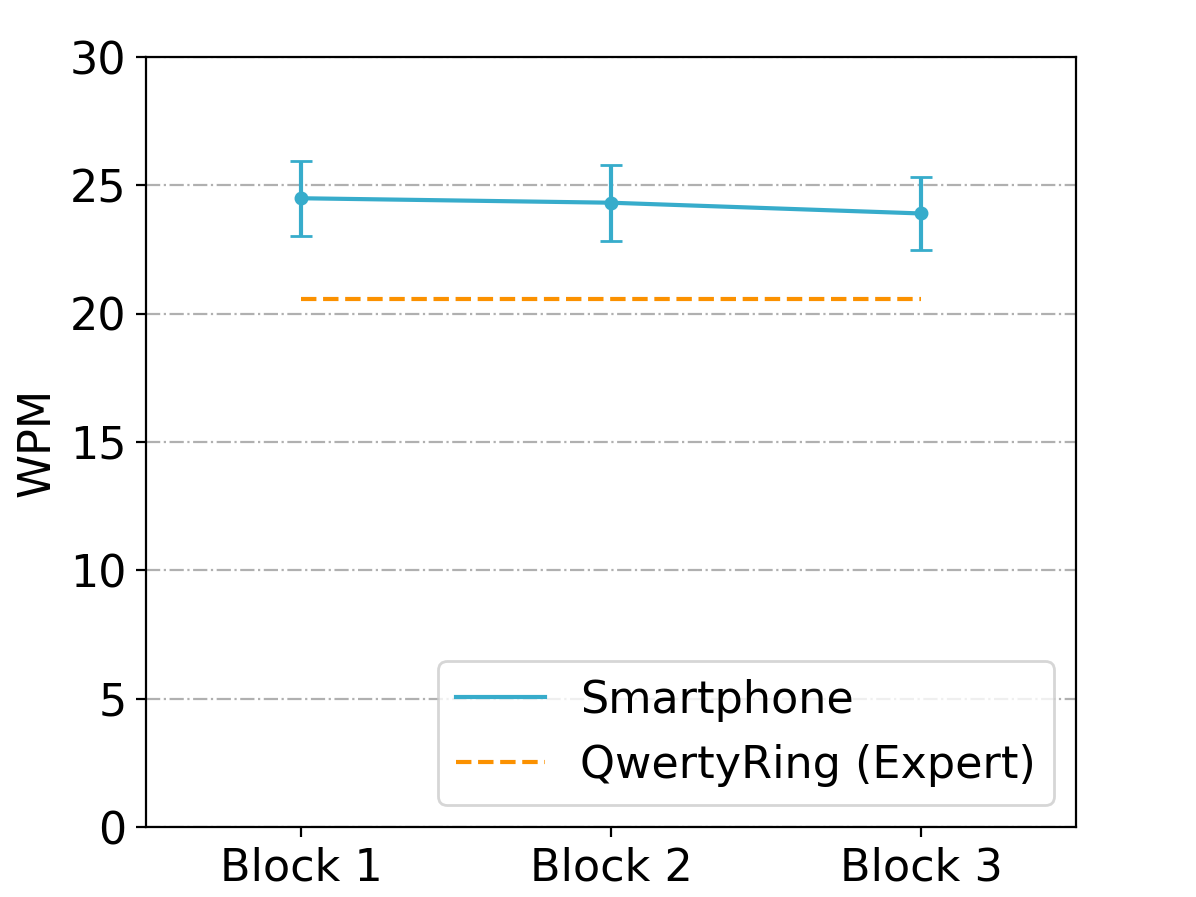
\includegraphics[width=0.8\linewidth]{figures/QwertyRing_vs_smartphone.png}
	\caption*{蓝线展示了被试在智能手机上食指打字的速度,误差条表示95\%置信区间。橙色虚线是QwertyyRing的专家打字速度,平均为蓝线的86.48\%。}
	\caption{比较智能打字指环与智能手指食指打字}
	\label{fig:QwertyRing_vs_smartphone}
\end{figure}

图\ref{fig:QwertyRing_vs_smartphone}展示了智能手机食指打字速度(蓝线)与智能打字指环专家打字速度的比较(橙线)。被试在三段实验中平均打字速度达到了23.81 WPM。方差分析表面实验段数对打字速度没有显著影响($F_{2,30}=0.20,p=.82$),也就是说,被试们已经达到了其手机食指打字速度的上线。智能打字指环的打字效率是这一结果的86.48\%,这表明智能打字指环提供了一种可穿戴的文本输入方法,而不会极大地牺牲打字速度。

\subsection{对评测结果的讨论}

\subsubsection{与其它文本输入技术比较}

智能打字指环的评测结果可以总结为:被试通过十分钟的热身练习,可以达到每分钟输入13.75个英文单词的打字速度,未纠正错误率为1.5\%;经过五天的练习后,被试可以达到每分钟输入20.59个英文单词的打字速度,未纠正错误率为1.3\%。这一表现明显优于现有的基于智能指环的文本输入技术。表格\ref{tab:QwertyRing_comparison}的上半部分将智能打字指环与现有智能指环文本输入相关论文进行了比较。表格中的新手指标(Novice)是各论文中第一时段实验的评测结果,专家指标(Expert)是最后一个时段实验的评测结果。其中,智能打字指环和\emph{RotoSwype}都进行了为期五天的用户实验,\emph{ThumbText}和\emph{TipText}进行了至少 40 分钟的用户实验,从表格中可以看出,智能打字指环在新手打字速度和专家打字速度上都有很大的优势。表格\ref{tab:QwertyRing_comparison}的下半部分展示了智能手机和智能手表上人们的平均打字速度,智能打字指环的表现接近智能手表上的打字速度,是智能手机上打字速度的三分之二。

\begin{table}[!htbp]
	\centering
	\begin{tabular}{l|llll}
		\toprule
		& \begin{tabular}[c]{@{}l@{}}\textbf{Novice}\\ \textbf{WPM}\end{tabular} & \begin{tabular}[c]{@{}l@{}}\textbf{Expert}\\ \textbf{WPM}\end{tabular} & \begin{tabular}[c]{@{}l@{}}\textbf{Novice}\\ \textbf{UER\%}\end{tabular} & \begin{tabular}[c]{@{}l@{}}\textbf{Expert}\\ \textbf{UER\%}\end{tabular} \\ \hline
		\textbf{智能打字指环 (通用化)}& \textbf{13.75} & \textbf{20.35} & \textbf{1.03}& \textbf{0.95}\\
		\textbf{智能打字指环 (个性化)}& \textbf{13.74} & \textbf{20.83} & \textbf{1.90}& \textbf{1.63}\\
		RotoSwype (指环) \cite{gupta2019rotoswype}    & 9.2& 14.8& 2.4& 0.5\\
		ThumbText (指环) \cite{kim2018thumbtext}          & 5.5& 11.4& 13.3& 9.1\\
		TypingRing (指环) \cite{nirjon2015typingring} & NA& 8.2& NA& NA\\
		TipText (指环) \cite{xu2019tiptext}          & 10.5 & 13.3 & 0.3 & 0.3\\ \hline
		Smartphone \cite{reyal2015performance}       & \multicolumn{2}{l}{30.3}& \multicolumn{2}{l}{2.4}\\
		Smartwatch \cite{gordon2016watchwriter}      & \multicolumn{2}{l}{22.0}& \multicolumn{2}{l}{1.5}\\
		\bottomrule
	\end{tabular}
	\caption{表格展示了智能打字指环与相关技术的对比。请注意,这一对比仅供参考,由于不同文献中的实验方法和实验条件不同,此对比不是完全公平的。}
	\label{tab:QwertyRing_comparison}
\end{table}

\subsubsection{学习效应}

智能打字指环用户需要将手腕贴在交互表面上,通过转动手腕来打字,用户需要适当的练习才能遵循此要求。在实验三的正式实验之前,有一个十分钟的热身阶段,实验者向被试介绍了智能打字指环的概念与用法,然后被试在实验者的指导下进行练习,并在十分钟的热身之后,达到了13.74 WPM的打字速度。这说明,智能打字指环是容易上手的。在为期五天的联系之后,被试达到了20.59 WPM的打字速度,而且学习曲线并没有收敛。这说明,若想使用智能打字指环达到专家级打字速度,需要较长的学习过程,但是专家打字速度非常快。

\subsubsection{通用化模型,还是个性化模型?}

实验三在各个方面对比了智能打字指环的通用化模型和个性化模型,无论在打字速度、打字准确率、单词解码器准确率和主观反馈上,两个模型都不存在显著性差异。原因有两点:首先,通用化模型已经能很好地预测用户所需单词了,因此个性化模型的改进空间有限;第二,单词解码器的改进对打字速度的提高而言不是很关键。实验三中对打字时间构成的分析已经说明,被试打字变快的主要原因是他们键入字母和选词的速度更快了,而单词解码器的改进对打字速度的帮助不大。尽管如此,在通用化模型和个性化模型的选择上,实验者仍然推荐个性化模型。这是因为,实验三已经发现,从第三天开始,个性化候选词解码器呈现出由于通用候选词解码器的趋势($p=.09$);被试的主观反馈也显示,他们感受到了个性化模型对单词解码准确率的改进。

\subsubsection{若指环佩戴在食指第一指骨会怎么样?}

在智能打字指环的交互设计中,实验者最终确定应当将指环佩戴在食指的第二指骨上。然而从社会接受程度的角度来说,各手指的第一指骨是更好的选择\cite{gu2019accurate},那么如果将指环佩戴在食指第一指骨上,智能打字指环的表现会怎么样呢?不幸的是,若指环佩戴在食指第一指骨上,智能打字指环将无法支持文本输入。具体来说,这一交互设计让指环无法区分想象键盘的第二行和第三行字母,因为这两种情况下惯性传感器的信号非常类似。实验者邀请实验三中四位专家用户(打字速度前四名)进行尝试,将指环佩戴在第一指骨上打字(单词解码器也针对该设置更新),他们甚至无法完整输入一句话,因为他们想要的单词往往不在候选词列表中。

当实验者将词库大小减少到 100 个单词时,四个参与者可以输入单词。在这种情况下,贝叶斯解码器可以找到所需的词,因此,在某些使用场景中,将智能打字指环佩戴在食指第一指骨上也是可行的:用户可以通过使用智能打字指环输入语义命令来触发智能手机上的快捷方式,如“播放音乐”。

\subsubsection{智能打字指环在其它无源表面上的表现}

智能打字指环单词解码器的准确率是本技术能否应用在一个无源表面上的关键,它受到两个因素的影响:(1)触摸事件识别的准确率;(2)触摸事件发生时手指运动信号是否能表征用户所想字母。实验者认为,智能打字指环支持任何类似桌面的无源表面上的输入文本,类似桌面的表面指的是坚硬的、平坦的、宽敞的表面:首先,实验二已经证明,触摸事件识别技术在类似桌面的交互表面(如木质和塑料桌子)上表现良好;第二,当用户在平坦的表面上打字时,其触摸时刻的手指运动信号应该与实验环境相似,而本技术在实验环境下的变现良好。

然后需要承认的是,智能打字指环无法支持软性表面的文本输入,以坐姿大腿上侧为例,大腿上侧不够平坦和宽敞,这会严重影响惯性传感指环的运动信号。实验者邀请了实验三的四名专家用户(打字速度前四名)参与非正式实验,评测他们使用智能打字指环在木质桌面、塑料桌面和大腿上侧的打字速度。四名被试在木质桌面上誊写10句话的速度是24.68 WPM(SD=4.13),在塑料桌面上打字速度为23.96 WPM(SD=2.42)。然而,被试们无法在大腿上侧完成所有的文本输入任务,因为一些想要的单词不在候选列表中。因此,大腿上侧基于惯性传感指环的触摸识别技术是可行的,但是基于指环的大腿上侧文本输入技术是不可行的。

\subsubsection{电量问题}

本章所介绍的内容默认以1000赫兹的惯性传感器信号作为基础,采用这一高频率信号的目的在于评测智能打字指环在最佳情况下的表现。然而,以1000赫兹的频率将惯性传感器数据发送到具有计算能力的机器上可能会很快地消耗智能指环的电量。有几种方法可以缓解电量问题:(1)首先,智能打字指环也可以在200赫兹的惯性传感信号下运行。实验二结果显示,触摸手势识别算法在200赫兹下运行良好。对于文本输入法单词解码器而言,200赫兹也是足够的,因为解码器只用到了传感器的俯仰角和偏航角等低频信息。(2)第二,商用的智能指环有开关,用户可以在不使用智能指环时关闭电源。在更理想的情况下,未来的研究者可以为智能指环开发一个低功耗模式,在用户可能进行文本输入时才切换至高功耗模式。

Oura Ring(https://ouraring.com/)是一个智能指环的例子,它比智能打字指环包含更多的传感器,包括红外接近光传感器、惯性传感器、体温传感器、蓝牙和电池。Oura Ring的电池重4到6克,宽7.9毫米,厚2.55毫米,一次充电可使用一周。相比之下智能打字指环所需的传感器更少,如果实现商业化,其电量问题也将得到解决。

\section{本章小结}

文本输入是重要的人机交互任务,然而,新型显示设备如增强现实头盔、智能电视等等,都面临文本输入效率不高的问题。本章提出了基于惯性传感指环的无源文本输入技术,该文本输入技术与显示设备解耦,用户只需佩戴智能指环,即可在任意无源表面上高效打字,这一特性使得该技术适用于各类显示设备,具有很强的普适性。利用触摸运动模型,惯性传感指环能够有效识别触摸交互中的触摸事件和抬起事件,准确率分别为99.30\%和99.50\%,还能准确分类多种触摸手势,如长按、滑动、左滑和右滑,准确率均高于99\%。实验者通过用户实验分析了被试使用惯性传感指环的打字行为,并据此设计了文本输入的单词解码器。在评测实验中,被试的上手打字速度为13.75 WPM,经过五天的练习后打字速度达到20.59 WPM。结果表明,基于惯性传感指环的无源表面文本输入技术易于学习,且打字效率远超其它智能指环文本输入技术,在增强现实、虚拟现实、智能电视等应用场景都具有实用价值。
